\documentclass{article} % For LaTeX2e
\usepackage{iclr2027_conference,times}

% Optional math commands from https://github.com/goodfeli/dlbook_notation.
\input{math_commands.tex}

\usepackage{hyperref}
\usepackage{url}

\usepackage{algorithm}      % algorithms
\usepackage{algorithmic}
\usepackage{amsmath}
\usepackage{tikz}
\usepackage{array}
\usepackage{booktabs}
\definecolor{WinGreen}{RGB}{120, 190, 120}     % ours wins
\definecolor{TieYellow}{RGB}{250,200,99}   % tie
\definecolor{LossRed}{RGB}{241,124,124}    % baseline wins
\usepackage{pgfplots}
\pgfplotsset{compat=1.18}
\usepackage{adjustbox}
\usepackage{caption}
\usepackage{amsmath}

\usepackage{amsthm}
\usepackage{amssymb}
\usepackage{mathabx}
\usepackage{subcaption}

\newtheorem{theorem}{Theorem}[section]
\newtheorem{lemma}[theorem]{Lemma}
\newtheorem{corollary}[theorem]{Corollary}

\theoremstyle{definition}
\newtheorem{definition}[theorem]{Definition}

\theoremstyle{remark}
\newtheorem{remark}[theorem]{Remark}

% Giảm khoảng trống trên/dưới bảng và hình
\setlength{\floatsep}{8pt plus 2pt minus 2pt}
\setlength{\textfloatsep}{10pt plus 2pt minus 2pt}
\setlength{\intextsep}{8pt plus 2pt minus 2pt}
\setlength{\abovecaptionskip}{4pt plus 1pt minus 1pt}
\setlength{\belowcaptionskip}{2pt plus 1pt minus 1pt}

\newcommand{\WinBar}[3]{%
\begin{tikzpicture}[baseline]
  \def\W{3.6}    % total width (cm)
  \def\H{0.5}   % height (cm) 
  \def\S{0.036}  % scale: 100 -> 3.6cm

  % bars
  \fill[WinGreen]   (0,0) rectangle (#1*\S,\H);
  \fill[TieYellow] (#1*\S,0) rectangle ({(#1+#2)*\S},\H);
  \fill[LossRed]   ({(#1+#2)*\S},0) rectangle (\W,\H);

  % outline
  % \draw[black, line width=0.3pt] (0,0) rectangle (\W,\H);

  % labels (only if wide enough)
  \ifdim #1pt>10pt
    \node[font=\scriptsize] at ({#1*\S/2},\H/2) {#1\%};
  \fi
  \ifdim #2pt>10pt
    \node[font=\scriptsize] at ({(#1+#2/2)*\S},\H/2) {#2\%};
  \fi
  \ifdim #3pt>10pt
    \node[font=\scriptsize] at ({\W-(#3*\S/2)},\H/2) {#3\%};
  \fi
\end{tikzpicture}%
}

\newcommand{\WinLegend}{%

\begin{tikzpicture}[baseline]
  \fill[WinGreen]   (0,0) rectangle (0.45,0.22);
  \node[anchor=west, font=\small] at (0.55,0.11) {Ours Wins};

  \fill[TieYellow] (2.5,0) rectangle (2.95,0.22);
  \node[anchor=west, font=\small] at (3.05,0.11) {Tie};

  \fill[LossRed]   (4.4,0) rectangle (4.85,0.22);
  \node[anchor=west, font=\small] at (4.95,0.11) {Baseline Wins};
\end{tikzpicture}
} 
\newcommand{\MethodCell}[2]{%
\begin{tabular}[c]{@{}l@{}}
#1\\
\textit{vs}\\
#2
\end{tabular}
}
\title{CONTRA-KD: Continuous Trajectory Alignment for Knowledge Distillation}

% Authors must not appear in the submitted version. They should be hidden
% as long as the \iclrfinalcopy macro remains commented out below.
% Non-anonymous submissions will be rejected without review.

\author{Antiquus S.~Hippocampus, Natalia Cerebro \& Amelie P. Amygdale \thanks{ Use footnote for providing further information
about author (webpage, alternative address)---\emph{not} for acknowledging
funding agencies.  Funding acknowledgements go at the end of the paper.} \\
Department of Computer Science\\
Cranberry-Lemon University\\
Pittsburgh, PA 15213, USA \\
\texttt{\{hippo,brain,jen\}@cs.cranberry-lemon.edu} \\
\And
Ji Q. Ren \& Yevgeny LeNet \\
Department of Computational Neuroscience \\
University of the Witwatersrand \\
Joburg, South Africa \\
\texttt{\{robot,net\}@wits.ac.za} \\
\AND
Coauthor \\
Affiliation \\
Address \\
\texttt{email}
}

% The \author macro works with any number of authors. There are two commands
% used to separate the names and addresses of multiple authors: \And and \AND.
%
% Using \And between authors leaves it to \LaTeX{} to determine where to break
% the lines. Using \AND forces a linebreak at that point. So, if \LaTeX{}
% puts 3 of 4 authors names on the first line, and the last on the second
% line, try using \AND instead of \And before the third author name.

\newcommand{\fix}{\marginpar{FIX}}
\newcommand{\new}{\marginpar{NEW}}

%\iclrfinalcopy % Uncomment for camera-ready version, but NOT for submission.
\begin{document}


\maketitle

\begin{abstract}
While Knowledge Distillation (KD) enables efficient compression of LLMs, current methods focus on matching discrete layer outputs, which fails to capture the continuous, dynamic nature of feature evolution within these models. We propose \textbf{CONTRA-KD}, a new paradigm for KD that reframes the process through continuous-time dynamics and the ordinary differential equations (ODE)-based nature of LLMs. We first learn a student-to-teacher correction flow in feature space using Rectified Flow, which provides a geometrically simple and stable transport path between intermediate representations. We then introduce a curriculum-based distillation strategy that guides the student to progressively follow this flow, targeting dynamic intermediate targets throughout the training process. This design enables the student to align not only with the teacher’s representations but also with its underlying feature dynamics, while remaining orthogonal and complementary to standard output-level distillation objectives. Extensive experiments across multiple teacher–student pairs and instruction-following benchmarks demonstrate that CONTRA-KD consistently improves distillation performance and training stability over strong baselines.
\end{abstract}

\section{Introduction}
Large Language Models (LLMs) have achieved remarkable capabilities, thanks to their immense scale with leading models now contain billions of parameters \cite{touvron2023llamaopenefficientfoundation}. However, this scale creates a substantial barrier for practical deployment, especially in constrained, low-resource settings. Knowledge Distillation \cite{hinton2015distillingknowledgeneuralnetwork} offers a compelling solution, by compressing a large, powerful teacher model into a smaller, faster student model by transferring knowledge between the two.

The dominant line of work distills LLMs purely at the level of final output distributions. The foundational recipe minimizes the forward KL divergence between the teacher and student output distributions \cite{hinton2015distillingknowledgeneuralnetwork,Bucila2006ModelC}. MiniLLM \cite{gu2024minillmknowledgedistillationlarge} instead optimizes reverse KL on student-generated samples, addressing the exposure-bias mismatch that arises under teacher-forced training. Building on this on-policy perspective, subsequent work explores a broader family of divergences and teacher--student distribution constructions, including generalized divergences, skewed objectives, contrastive formulations, and adaptive intermediate distributions \cite{agarwal2024onpolicydistillationlanguagemodels,ko2024distillmstreamlineddistillationlarge,ko2025distillm2contrastiveapproachboosts,shin2026amid}. Other recent studies focus on the sampling and data-generation process itself, using interleaved student--teacher generation or difficulty-aware data selection to reduce the teacher--student mismatch \cite{xu2025speculative,pmlr-v267-he25c}. Despite these refinements, the supervision signal in this family remains fundamentally anchored to the model's final output: whether the divergence is measured on probabilities, logits, or student-generated rollouts, the internal computation that transforms one representation into another remains largely unconstrained. 

Grounded in the theory of Ordinary Differential Equations (ODEs), this motivates the interpretation of treating the layer-wise progression of a Transformer as a sequence of discrete time steps in a continuous evolution of feature representations \cite{chen2019neuralordinarydifferentialequations,tong2025neural}. Under this lens, the teacher's deeper architecture can be viewed as a fine-grained numerical solver tracing a detailed path through feature space, while the student's shallower architecture acts as a coarser solver that attempts to approximate the same underlying trajectory. A growing line of work has begun to target this internal computation directly rather than supervising only the output layer. Representation-based approaches align hidden states, attention structure, or relational geometry across selected layers, while more recent methods improve robustness to architectural or dimensional mismatch and account for residual discrepancies between teacher and student representations \cite{zhang2024dualspaceknowledgedistillationlarge,dasgupta2025improving,on2026knowledge}. Beyond matching individual states, recent work has explicitly considered the dynamics of intermediate features, supervising layer-to-layer changes in addition to hidden representations and aligning trajectories at multiple granularities \cite{gong-etal-2025-beyond,chi-etal-2026-mta}. These developments are important because they move distillation from output imitation toward supervision of the computation itself. Nevertheless, the teacher's trajectory is still represented through a finite collection of layer checkpoints: states, finite differences, or relational structures are evaluated at selected depths, while the transformation connecting neighboring states is not modeled explicitly. The geometry of how a representation is transported between observed checkpoints therefore remains largely unconstrained. Concurrently, the emerging literature on continuous-time flow matching \cite{lipman2023flowmatchinggenerativemodeling,liu2022flowstraightfastlearning} provides a natural mechanism for learning such continuous transformations through a velocity field that transports one distribution toward another. This perspective complements the ODE view of Transformers introduced above: \textit{distillation can be recast as learning a continuous transport process that guides the student's representations along a trajectory consistent with the teacher's flow.} 

Grounded in this insight, we introduce \textbf{CONTRA-KD}, a new framework that formulates KD as a rectified flow matching problem in feature space. Rather than forcing the student to replicate the teacher's full and often noisy dynamics, CONTRA-KD first learns an idealized rectified flow: a straight-line ODE capturing the most direct transformation from a student's feature state to its corresponding teacher state. We prove that minimizing this trajectory discrepancy also bounds the discrepancy between the two models' underlying velocity fields, so distilling the hidden-state flow alone implicitly carries the teacher's dynamics to the student, without ever matching velocities directly. However, matching a distant, information-rich teacher state from the start of training produces noisy, unstable updates. We therefore guide the student along the flow through a curriculum, aligning short segments first and lengthening them as training progresses. In the second stage, the student aligns its own layer-wise updates with a discretized simulation of this flow, replacing brittle, discrete state matching with a continuous dynamical perspective.

The contributions of our study are as follows:
\begin{itemize}
    \item We show that trajectory alignment implicitly induces dynamic alignment: minimizing the discrepancy between student and teacher hidden-state trajectories bounds the discrepancy between their governing velocity fields, so that distilling the continuous flow is sufficient to transfer the teacher's underlying dynamics.
    \item We propose a new framework, Continuous Trajectory Alignment for Knowledge Distillation (\textbf{CONTRA-KD}). CONTRA-KD first learns a universal, student-to-teacher correction flow. In the second stage, the student is trained via a discretized simulation of this rectified flow, using it as a dynamic target for more stable and efficient feature evolution. We further extend this design to the cross-tokenizer scenario, enabling distillation between teacher-student pairs with different vocabularies.
    \item We show that trajectory alignment without a curriculum is unstable, as forcing the student to match distant, information-rich teacher states early in training destabilizes optimization. This motivates \textbf{curriculum-based trajectory distillation}, which progressively increases distillation difficulty by distilling small-step dynamics first and gradually extending the step size, stabilizing optimization and enabling effective velocity and trajectory alignment.
\end{itemize}


\section{Preliminary}

% \subsection{Related work}
% \paragraph{Knowledge distillation of LLMs.} Knowledge Distillation (KD) \cite{hinton2015distillingknowledgeneuralnetwork} is a model compression technique where a student learns from a teacher model's outputs. A line of research has focused on treating distillation as a sequence-level alignment problem \cite{kim2016sequencelevelknowledgedistillation}. More recent methods have built on this, by using Kullback–Leibler divergence on student generated outputs (SGOs) \cite{lin2020autoregressiveknowledgedistillationimitation}, employing Jensen-Shannon divergence \cite{agarwal2024onpolicydistillationlanguagemodels}, or Reverse KLD \cite{gu2024minillmknowledgedistillationlarge, wu2024rethinkingkullbackleiblerdivergenceknowledge}.

% \paragraph{Intermediate representations distillation.} A complementary line of work explores distilling knowledge from a teacher’s intermediate representations, motivated by the observation that deep models encode rich hierarchical information beyond their outputs \cite{skean2025layerlayeruncoveringhidden}. Early successes in this direction were demonstrated for BERT-style architectures \cite{sanh2020distilbertdistilledversionbert, jiao2020tinybertdistillingbertnatural}. More recently, inspired by interpreting Transformers as discretizations of Ordinary Differential Equations (ODEs) \cite{chen2019neuralordinarydifferentialequations, lu2019understandingimprovingtransformermultiparticle}, feature dynamics distillation methods have framed KD as aligning the trajectories of a coarse ODE solver (the student) with those of a fine-grained solver (the teacher) \cite{gong-etal-2025-beyond}. While conceptually appealing, these approaches rely on discrete layer-to-layer differences as proxies for continuous dynamics, which can limit their ability to capture the global geometry of the teacher’s feature flow.

% \textbf{Generative Modeling Perspectives on KD.} Parallel to advances in LLM distillation, generative modeling has increasingly been explored as a vehicle for knowledge transfer. In vision and multimodal domains, diffusion-based and score-matching models have been distilled by training student models to approximate a teacher’s generative process, for instance by matching denoising trajectories or regressing score functions \cite{huang2023knowledgediffusiondistillation, yao2024progressivekd}. In a complementary line of work, flow-based and rectified flow models \cite{liu2022flowstraightfastlearning, lipman2023flowmatchinggenerativemodeling} introduce deterministic ODE formulations that learn vector fields transporting samples between distributions along simple paths, enabling efficient distillation without reliance on stochastic sampling. Collectively, these methods demonstrate that learning simplified, geometry-aware transport dynamics can preserve essential generative behavior while substantially reducing model complexity.

% While these methods are powerful, their primary focus remains on the model's final output, overlooking the richer intermediate representation of LLMs \cite{skean2025layerlayeruncoveringhidden}. An alternative and complementary perspective is to distill the knowledge encoded in model's intermediate layers. While studies focus on BERT-based models show the potential of this scheme \cite{sanh2020distilbertdistilledversionbert, jiao2020tinybertdistillingbertnatural}, recent prominent works, motivated by viewing the intepretation of Transformers as a discretized Ordinary Differential Equations (ODEs) \cite{chen2019neuralordinarydifferentialequations, lu2019understandingimprovingtransformermultiparticle}, see distillation as a problem of aligning the feature dynamics of a coarse ODE solver (the student) with a fine-grained one (the teacher) \cite{gong-etal-2025-beyond}. While being novelty, this work relies on discrete, layer-to-layer changes to approximate the true continuous flow of information. Our work aims to address this by applying tools from continuous time generative models \cite{liu2022flowstraightfastlearning, lipman2023flowmatchinggenerativemodeling}, learning an ODE that transforms between two distributions by directly regressing a vector field onto a target (teacher) path. Having learned this straight-path correction flow, we distill this simplified signal to the student. 

% \subsection{Preliminary}
\subsection{Knowledge distillation in LLMs}
Knowledge distillation (KD) \cite{hinton2015distillingknowledgeneuralnetwork} is a technique for model compression where a large teacher model transfers its knowledge to a smaller student model. The conventional KD framework primarily achieves this by aligning the final output distributions (logits) of the student with those of the teacher. Specifically, for a final-layer student hidden state $h_S^{L_S}$ and teacher hidden state $h_T^{L_T}$, where the student and the teacher have $L_S$ and $L_T$ layers respectively, the loss minimizes the Kullback-Leibler (KL) divergence between the probability distributions produced by their respective language modeling heads, $f_{\text{head}}(\cdot)$:
\begin{equation}
\mathcal{L}_{KD}=\mathbb{E}_{x\sim data}[D_{KL}(f_{head}^{T}(h_{T}^{L_{T}})||f_{head}^{S}(h_{S}^{L_{S}}))]
\end{equation}

However, this approach often fails to capture the rich information encoded within the immediate representations of LLMs. Feature Dynamic Distillation (FDD) \cite{gong-etal-2025-beyond} addresses this limitation by framing the distillation problem as aligning the entire feature dynamics between models, including additional loss term that match both the feature trajectory and its first-order derivative. Our work further extends this approach to a continuous path-based approach to feature-space alignment. 

\subsection{Dynamic perspective of LLMs}
A foundational perspective for neural networks is to view their discrete, layer-wise structure as an Euler discretization of a continuous-time system governed by an ordinary differential equation (ODE) \cite{chen2019neuralordinarydifferentialequations}. In this paradigm, a neural network is not a sequence of layers but a model that parameterizes a continuous vector field. This vector field defines the instantaneous rate of change of the hidden state: $\frac{d\textbf{h(t})}{dt} = f\big(h(t), t, \theta\big)$. From this dynamic perspective, a student model can be seen as a coarse discretization of the feature dynamics, where a larger model represents a finer representation of the same process \cite{gong-etal-2025-beyond}. This suggests that effective knowledge transfer should align the underlying continuous dynamics that govern feature evolution.
%% need extension

\subsection{Continuous-time flow-based models}
Continuous Normalizing Flows transform a prior distribution $p_0$ into a target distribution $p_1$ via a time-dependent vector field $u_t$, with the flow $\phi_t(x)$ following the ODE $\frac{d}{dt}\phi_t(x) = u_t(\phi_t(x))$, $\phi_0(x) = x$. Since the marginal path induced by this ODE is intractable to model directly, Flow Matching \cite{lipman2023flowmatchinggenerativemodeling} instead trains a neural vector field $v_\theta$ to regress the velocity of a tractable conditional interpolation path $X_t = \psi_t(x_0, x_1)$ between paired samples $(x_0, x_1) \sim \pi$. Rectified Flow \cite{liu2022flowstraightfastlearning} instantiates this idea with a linear interpolation path, $X_t = (1-t)x_0 + tx_1$, under which the conditional velocity field becomes the constant vector $x_1 - x_0$, reducing the objective to a simple least-squares regression:
\begin{equation}
\mathcal{L}_{\text{RF}}(\theta) = \mathbb{E}_{t\sim\mathcal{U}(0,1),\, (x_0,x_1)\sim\pi}\left[\|(x_1-x_0) - v_\theta(X_t,t)\|^2\right].
\end{equation}
This construction induces straight-line trajectories in Euclidean space and admits exact simulation with a single Euler step, providing a geometrically principled and computationally efficient foundation that we later leverage for feature-space alignment in CONTRA-KD.

\section{Method}
% This section details our proposed framework CONTRA-KD. We first show that by learning the flow between teacher and student hidden states, we can distill not only the intermediate representations but also their internal dynamics in Section \ref{sec:motivation}. In particular, we will construct the teacher-student flow in Section \ref{sec:flow_construct}. Section \ref{sec:distill} and \ref{sec:final_loss} will elaborate how to apply CONTRA-KD design into distillation process and incorporate with existing methods.

\subsection{Our Motivation}
\label{sec:motivation}
\paragraph{Trajectory alignment implies dynamic alignment.} Under the perspective of continuous-time paradigm, the teacher and student models are dynamic systems over layer index $t$\footnote{Here, $t$ implies the continuous time variable over which the hidden representations transform; it is equivalent to the discrete layer indices of Transformer models.} governed by distinct velocity fields. Let the teacher's and student's evolution be governed by velocity fields $v_T$ and $v_S$. Their hidden state trajectories, $h_T(t)$ and $h_S(t)$\footnote{$h_T(t)$ and $h_S(t)$ are indeed $h_T(x,y, t)$ and $h_S(x,y, t)$ where $(x,y)$ represents a pair of input and output sampled from the ground-truth data distribution. We ignore them for brevity.}, are solutions of:
\begin{equation}
\frac{dh_{T}(t)}{dt}=v_{T}(h_{T}(t),t); \quad \frac{dh_{S}(t)}{dt}=v_{S}(h_{S}(t),t)
\end{equation}

To ensure robust knowledge transfer, the student must learn from the teacher's internal dynamics. Mathematically, this is equivalent to minimizing the difference between the trajectories generated by their respective vector fields:
\begin{align}
 & \mathbb{E}_{t\sim U\left(0,1\right)}\left[\Vert h_{T}\left(t\right)-h_{S}\left(t\right)\Vert_{\mathcal{L}_{2}}\right]
 =\mathbb{E}_{t\sim U\left(0,1\right)}\left[\left[\int_{\Omega}\left[h_{T}\left(t;x,y\right)-h_{S}\left(t;x,y\right)\right]^{2}dxdy\right]^{1/2}\right],
\end{align}
where $\Omega$ is the domain of $(x,y)$. 

Let us denote $\delta_{t}=v_{S}\left(h_{T}\left(t\right),t\right)-v_{T}\left(h_{T}\left(t\right),t\right)$. In the following theorem, we prove that the trajectory distillation can lead to the dynamic or velocity distillation. 

\begin{theorem}
  \label{def:inj}
Assume that the teacher and student velocities satisfy $M$-Lipchitz. We have the following inequality:
\begin{equation}
\label{eq:delta_bound}
\Vert\delta_{t}\Vert_{\mathcal{L}_{2}} \leq M\Vert h_{T}\left(t\right)-h_{S}\left(t\right)\Vert_{\mathcal{L}_{2}}
 +\Vert\frac{d}{dt}\left[h_{S}\left(t\right)-h_{T}\left(t\right)\right]\Vert_{\mathcal{L}_{2}},
\end{equation}
where $\Vert f\Vert_{\mathcal{L}_{2}}:=\left(\int f\left(a\right)^{2}da\right)^{1/2}$.
\end{theorem}

The detailed theoretical proof is provided in Appendix \ref{app:proof}. Equation \eqref{eq:delta_bound} shows a direction connection between trajectory alignment and velocity alignment, which bounds the dynamic difference $\delta_t$ in terms of the trajectories and its rate of change. When the student is trained to distill the teacher's hidden states, the state difference $\Vert h_{T}\left(t\right)-h_{S}\left(t\right)\Vert_{\mathcal{L}_{2}}$ and its temporal derivative $\Vert\frac{d}{dt}\left[h_{S}\left(t\right)-h_{T}\left(t\right)\right]\Vert_{\mathcal{L}_{2}}$ are driven to 0. Consequently, the dynamic or velocity difference $\delta_t$ also converges to 0. This implies that matching the trajectories implicitly enforces the student's dynamics to follow the teacher's dynamics. Therefore, trajectory distillation leads to dynamic distillation, ensuring the student not only reproduces the teacher's states but also learns its underlying dynamics.

\paragraph{Curriculum learning through continuous flow.} While Theorem \ref{def:inj} shows that aligning student and teacher trajectories implicitly enforces dynamic alignment, directly matching trajectories can be difficult, especially at early training stages when the student's representations are far from teacher's. This motivates a curriculum-based strategy, where the student is not forced to immediately match the teacher's states but instead progress toward them through a sequence of intermediate targets (Figure \ref{fig:curriculum_learning}). To realize this curriculum, we define a \textit{straight flow} connecting corresponding representations of student and teacher, where intermediate states of this flow serve as progressively easier alignment targets. As training progresses, the step size is gradually increased, enables the student to traverse longer segments and progressively approach teacher's trajectory. Further analysis can be found in Section \ref{sec:ablation_cl}.

\begin{figure}[t]
\centering
\begin{minipage}[c]{0.42\linewidth}
    \centering
    \includegraphics[width=\linewidth]{illustration/contra-flow.png}
\end{minipage}
\hfill
\begin{minipage}[c]{0.55\linewidth}
    \refstepcounter{figure}\label{fig:curriculum_learning} 
    \textbf{Figure \thefigure:} 
    \textbf{Curriculum learning through continuous flow.} The blue line denotes teacher trajectories, the red line denotes student trajectories, and the dotted gray arrow indicates our learned student--teacher flow. In early step of training, the student follows a short segment of this flow with an intermediate target that is easier to optimize, and gradually increases the step sizes as training progresses.
\end{minipage}
\vspace{-1.5em}
\end{figure}

\subsection{Student-Teacher Continuous Flow} 
\label{sec:flow_construct}
Formally, let $h_S^j \in \mathbb{R}^{N \times d_S}$ and $h_T^j \in \mathbb{R}^{N \times d_T}$ be the feature representations coming out from a selected intermediate layer $j$ of a student and teacher model, respectively, for a given input with sequence length $N$. Typically, they reside in spaces of different dimensions. With the assumption that the teacher's hidden space is better trained and can express more information, we first project the student's hidden states to the teacher's space and use these projected hidden states for later steps. This projection can be parameterized as simple as a weight matrix $W^{S \xrightarrow{} T} \in \mathbb{R}^{d_S \times d_T}$:
\[
f_{\text{proj}} (h_S^j) := h_S^j W^{S \xrightarrow{} T} \in \mathbb{R}^{N \times d_T}
\]
A second challenge is the mismatch in the number of layers ($L_S \neq L_T$). To tackle this, we use a uniform layer scheduling schema by selecting a subset of $L_D$ layers from both the student and the teacher and form pairs of aligned layers. We denote $I_S = \{l_1^S, l_2^S, ..., l_{L_D}^S\}$ and $I_T = \{l_1^T, l_2^T, ..., l_{L_D}^T\}$ as the ordered sets of selected layer indices for the student and the teacher, respectively.

The transformation is modeled as the trajectory of a time-dependent ODE, where for the $i$-th token and the $j$-th layer pair in our schedule, a continuous state $Z_t^{(i,j)}$ evolves from $t=0$ to $t=1$ according to:
$\frac{d Z_t^{(i,j)}}{dt} = v_\theta(Z_t^{(i,j)}, t, j)$. The trajectory starts at the student's distribution $Z_0^{(i,j)}$ and is guided to the teacher's distribution $Z_1^{(i,j)}$. We denote $Z_0^{(i,j)} := h_S^{j}[i]$ as the student's hidden representation of the $i$-th token in the token sequence at the $j$-th aligned layer (i.e., the $l_j^S$-th layer in the student model) and, similarly, $Z_1^{(i,j)} := h_T^{j}[i]$ as the teacher's hidden representation of the same token at the teacher's $l_j^T$-th layer. The neural network  $v_\theta$, conditioned on distillation step index $j$, parameterizes the dynamics of this transformation, learning the direction and magnitude of feature correction at any intermediate point $(Z_t)$ along the path.

\begin{minipage}[t]{0.4\textwidth}
\vspace{0pt}
In Euclidean geometry of feature spaces, the straight path is the shortest possible route between two endpoints and can be simulated without time discretization. Therefore, we constrain our learned ODE to follow this trajectory. To achieve this, we apply the learning objective of Rectified Flow. For any pair of corresponding states $(h_S^{j}[i], h_T^{j}[i])$, we define a linear interpolant $H_t^{(i, j)}$:
\begin{equation}
H_t^{(i,j)} := (1-t)\, h_S^{j}[i] + t\, h_T^{j}[i]
\end{equation}
The target velocity vector required to traverse this path is a constant vector, that is, the vector from the student's state to the teacher's state: 
\begin{equation}
\frac{d H_t^{(i,j)}}{dt} = h_T^{j}[i] - h_S^{j}[i]
\end{equation}
\end{minipage}
\hfill
\begin{minipage}[t]{0.58\textwidth}
\vspace{-1em}
\begin{algorithm}[H]
  \caption{Training the Velocity Field $v_\theta$}
  \label{alg:train_v_theta}
  \begin{algorithmic}[1]
    \STATE \textbf{Input:} teacher $p$, student $q$, projector $f_{\text{proj}}$, velocity field $v_\theta$ with parameter $\theta$, data $\mathcal{D}$, layer maps $I^S, I^T$
    \STATE \textbf{Output:} Trained velocity field $v_\theta$
    \FOR{each batch $\{x_i\}$ in $\mathcal{D}$}
      % \STATE $j \sim U\{1, \ldots, L_D\}$
      \STATE Initialize $\mathcal{L}(\theta) \gets 0$
      \FOR{$j = 1,2,...,L_D$}
      \STATE $h_S^j \gets f_{\text{proj}}\!\left(q(\{x_i\}, \text{layer}=l_j^S)\right)$
      \STATE $h_T^j \gets p(\{x_i\}, \text{layer}=l_j^T)$
      \STATE $t \sim U(0,1)$
      \STATE $H_t^j \gets (1 - t)\cdot h_S^j + t\cdot h_T^j$
      \STATE $\mathcal{L}(\theta) \gets \mathcal{L}(\theta) + \left\| (h_T^j - h_S^j) - v_\theta(H_t^j, t, j) \right\|^2$
      \ENDFOR
      \STATE Update $\theta$ using gradients from $\mathcal{L}(\theta)$
    \ENDFOR
    \STATE \textbf{return} $v_\theta$
  \end{algorithmic}
\end{algorithm}
\end{minipage}

Our goal is to train a velocity field network $v_\theta$ that perfectly replicates this target vector field. The learning objective for $v_\theta$ for an input data sample is as follows:
\begin{equation}
\mathcal{L}(\theta) = \mathbb{E}_{i, j, t} \left[ \left\| \left(h_T^{j}[i] - h_S^{j}[i]\right) - v_\theta\left(H_t^{(i,j)}, t, j\right) \right\|^2 \right]
\end{equation}
The expectation is taken over sequence of tokens $i$, distillation steps $j \in \{1, ..., L_D\}$, and time steps $t \sim U(0,1)$. The overall training procedure of the velocity field is detailed in Algorithm~\ref{alg:train_v_theta}.
% \subsection{Distillation as a Continuous Feature Transformation}
\subsection{Curriculum-based Trajectory Distillation}
\label{sec:distill}
\paragraph{Curriculum-based approach. }Directly distilling the teacher trajectory by alignment between $\phi_0(h_S) = h_S$ and $\phi_1(h_S) = h_T$ can be challenging at early stages of training, where the student representation is still far from the teacher's and can lead to unstable update signals. To address this issue, we introduce a \textbf{curriculum-based trajectory distillation} strategy that effectively ultilizes supervision from the learned flow.

Specifically, for a flow $\phi_t(x)$ and corresponding velocity field $u_t$, we define an intermediate target $\tilde{\phi}_k(x)$ at time step $k$ from $\phi_0(x) = x$, where $k \in (0, 1]$. Intuitively, $\tilde{\phi}_k(x)$ lies partway along the flow induced by $u_t$ at distance defined by $k$ rather than the endpoint $\phi_1(x)$. The target can be effectively approximated by: $\tilde{\phi}_k(x) := {\phi_0(x)} + \int_{0}^{k} u_t(\phi_t(x)) \, dt$. For a smaller value of $k$, the target is easier to follow, forming a curriculum that progressively increases in difficulty as training proceeds.

\paragraph{Distillation process. } Let
$h_S^{j}[i]$ denote the projected hidden representation of the $i$-th token at the $j$-th aligned layer for a data sample. The corresponding curriculum-based target is defined as an Euler step from the student's representation:
\begin{equation}
  \tilde{h}_S^{j}[i] := \mathrm{sg}\left[ h_S^{j}[i] + k \cdot v_\theta\left(h_S^{j}[i],\, t=0,\, j\right) \right],
  \label{eq:dynamic_target}
\end{equation}
where $\mathrm{sg}[\cdot]$ denotes the stop-gradient operator. During training, \(k\) is gradually increased based on training iterations: $k=\frac{t}{T}$, where $t$ is the iteration index and $T$ is the total number of training iterations. The CONTRA loss then minimizes the discrepancy between the student's layer output and this dynamically generated target:
\begin{equation}
\mathcal{L}_{\text{CONTRA}} = \frac{1}{N L_D} \sum_{j=1}^{L_D} \sum_{i=1}^{N} D_{\text{cos}}\left( h_S^{j}[i],\, \tilde{h}_S^{j}[i] \right)
\end{equation}

Because $\tilde{h}_S^{j}[i]$ is detached, minimizing $D_{\text{cos}}(h_S^{j}[i], \mathrm{sg}[\tilde{h}_S^j[i]])$ forces the gradient of $h_S^j[i]$ to align with the vector direction prescribed by $v_\theta(h_S^j[i], 0, j)$. This updates the student hidden state along the local tangent of the Rectified Flow vector field toward the teacher representation space. We employ cosine distance over $\ell_2$ distance to focus optimization on directional alignment, avoiding gradient instability in high-dimensional feature spaces. To prevent distributional shift between the student and the learned flow, we alternate between updating the student on $\mathcal{L}_{\text{CONTRA}}$ and re-adapting $v_\theta$ and $f_{\text{proj}}$ following Algorithm~\ref{alg:contra_distillation}.
% where $D_{\text{cos}}(a, b) = 1 - \frac{a^T \cdot b}{\|a\| \|b\|}$ is the cosine distance between 2 vectors. We adopt the cosine distance as it emphasizes directional alignment of student updates with the rectified flow. To avoid distribution shift when updating the student model, we continue to train the velocity field and the projector after each distillation epoch, alternating between updating the student on $\mathcal{L}_{\text{CONTRA}}$ and re-adapting $v_\theta$ and $f_{\text{proj}}$ following Algorithm~\ref{alg:train_v_theta}. The full two-phase training loop is detailed in Algorithm~\ref{alg:contra_distillation} in Appendix~\ref{app:contra_algo}.
\subsection{Cross-tokenizer Mechanism}

% To ensure our method's robustness, we extend from the same-tokenizer scenario to enable knowledge distillation between cross-tokenizer, cross-architecture teacher-student pairs. Similar to state-of-the-art KD methods, the main issue when applying our method to cross-tokenizer KD is the sequence length mismatch between teacher and student due to different vocabularies. We employ a strategy that identifies sequences of tokens that represent the same piece of text, called a "token span", and perform distillation at the span level which ensures matching sequence lengths.

\paragraph{Span Construction via Longest Common Subsequence.}
When teacher and student use different tokenizers, their tokenizations of the same input $x$ produce sequences of different lengths, making direct token-level alignment infeasible. To
resolve this, we note that both tokenizers operate over the same character stream, so each
token can be annotated with its character-level end offset. This gives two offset sequences $\mathbf{o}^T = (\mathrm{off}^T_1, \ldots, \mathrm{off}^T_{n_T})$ and $\mathbf{o}^S = (\mathrm{off}^S_1, \ldots, \mathrm{off}^S_{n_S})$ for the teacher and student, respectively. Special tokens are assigned offset $0$ and excluded from alignment. In addition to LCS, we also investigate an alternative edit-distance alignment strategy in Appendix \ref{app:edit_distance_alignment}.

We compute the Longest Common Subsequence (LCS) of $\mathbf{o}^T$ and $\mathbf{o}^S$ to identify shared character boundaries, which define the start and end token indices of a span
in each model. This produces $N_\mathrm{sp}$ aligned span pairs:
\begin{equation}
    \mathcal{M}_s = \bigl\{(\mathrm{Span}^S_i,\, \mathrm{Span}^T_i)\bigr\}_{i=1}^{N_\mathrm{sp}},
    \quad \mathrm{Span}^\cdot_i = (s^\cdot_i,\, e^\cdot_i),
\end{equation}
where $s^\cdot_i$ and $e^\cdot_i$ are the start and end token indices of span $i$. 

\paragraph{Span Representation.}
For each aligned span pair, we form span-level representations by mean-pooling the token hidden states within each span. At aligned layer $j$, the student and teacher span representations are:
\begin{equation}
    C^{S,(j)}_i = \frac{1}{e^S_i - s^S_i + 1} \sum_{t=s^S_i}^{e^S_i} f_\mathrm{proj}(h^{j,S}_t),
    \qquad
    C^{T,(j)}_i = \frac{1}{e^T_i - s^T_i + 1} \sum_{t=s^T_i}^{e^T_i} h^{j,T}_t,
\end{equation}
where $f_\mathrm{proj}$ projects the student hidden states into the teacher's feature space. Since the two span sequences now have equal length $N_\mathrm{sp}$, we can apply trajectory alignment at the span level.

% \paragraph{Span-Level Trajectory Loss.}
% We define a linear interpolant between corresponding span representations and train $v_\theta$ to predict the direction from student to teacher:
% \begin{equation}
%     \mathcal{L}_\mathrm{RF} = \mathbb{E}_{i,j,t}\Bigl[
%         \bigl\|(C^{T,(j)}_i - C^{S,(j)}_i) - v_\theta(\mathcal{H}^{(i,j)}_t,\, t,\, j)\bigr\|^2
%     \Bigr], \quad \mathcal{H}^{(i,j)}_t = (1-t)\,C^{S,(j)}_i + t\,C^{T,(j)}_i.
% \end{equation}
% The curriculum-based distillation target for span $i$ at layer $j$ is then:
% \begin{equation}
%     \tilde{C}^{S,(j)}_i = C^{S,(j)}_i + k \cdot v_\theta(C^{S,(j)}_i,\, t{=}0,\, j),
% \end{equation}
% where $k \in (0,1]$ grows progressively during training. The CONTRA loss minimizes the
% cosine distance between the student span state and this target:
% \begin{equation}
%     \mathcal{L}_\mathrm{CONTRA} = \frac{1}{N_\mathrm{sp} L_D}
%     \sum_{j=1}^{L_D} \sum_{i=1}^{N_\mathrm{sp}}
%     D_\mathrm{cos}(C^{S,(j)}_i,\; \tilde{C}^{S,(j)}_i).
% \end{equation}

\subsection{Final Objective Function}
\label{sec:final_loss}
A key advantage of CONTRA-KD is its orthogonality to existing distillation objectives. It acts as a complement on internal feature space, while other methods utilizing KD loss terms focus on output logits. Therefore, we integrate $\mathcal{L}_{\text{CONTRA}}$ as a complementary term to standard KD baselines. The final loss function is the sum of these components; note that $\mathcal{L}_{CONTRA}$ here is computed per sample and averaged over all samples in a batch:
\begin{equation}
\mathcal{L} = \mathcal{L}_{CE} + \mathcal{L}_{KD} + \mathcal{L}_{CONTRA}
\end{equation}
\section{Experiments}
\begin{table}[t]
\centering
\caption{Win / Tie / Loss rates (\%) across student-teacher pairs on different benchmark datasets, evaluated by \texttt{GPT-4o-mini}. \textbf{Win} indicates preference for \textsc{CONTRA-KD} (Ours Win), \textbf{Loss} indicates baseline preference, and \textbf{Tie} denotes equal quality.}
\label{tab:winrates}
\small
\setlength{\tabcolsep}{3.5pt}
\resizebox{\linewidth}{!}{%
\begin{tabular}{l ccc ccc ccc}
\toprule
& \multicolumn{9}{c}{\textbf{Evaluation Set}} \\
\cmidrule(lr){2-10}
\textbf{Method}
& \multicolumn{3}{c}{\textit{Dolly}}
& \multicolumn{3}{c}{\textit{Self-Instruct}}
& \multicolumn{3}{c}{\textit{Vicuna}} \\
\cmidrule(lr){2-4} \cmidrule(lr){5-7} \cmidrule(lr){8-10}
& Win & Tie & Loss
& Win & Tie & Loss
& Win & Tie & Loss \\
\midrule
\multicolumn{10}{c}{\textit{OpenLLaMA2 7B $\rightarrow$ 3B}} \\
\midrule
DistiLLM (+CONTRA vs.\ baseline)    & \textbf{41.24} & 21.80 & 36.96 & \textbf{41.98} & 19.67 & 38.35 & \textbf{45.50} & 14.25 & 40.25 \\
FDD (+CONTRA vs.\ baseline)         & \textbf{42.32} & 21.24 & 36.44 & \textbf{44.27} & 17.47 & 38.26 & \textbf{43.75} & 15.50 & 40.75 \\
DistiLLM-2 (+CONTRA vs.\ baseline)  & \textbf{40.28} & 23.10 & 36.62 & \textbf{39.67} & 25.78 & 34.55 & \textbf{45.50} & 11.00 & 43.50 \\
CSD (+CONTRA vs.\ baseline)         & \textbf{42.68} & 22.28 & 35.04 & \textbf{40.39} & 24.98 & 34.63 & \textbf{44.75} & 18.50 & 36.75 \\
\midrule
\multicolumn{10}{c}{\textit{GPT2 1.5B $\rightarrow$ 0.1B}} \\
\midrule
DistiLLM (+CONTRA vs.\ baseline)    & \textbf{38.32} & 31.24 & 30.44 & \textbf{35.37} & 34.15 & 30.48 & \textbf{38.25} & 31.50 & 30.25 \\
FDD (+CONTRA vs.\ baseline)         & \textbf{34.28} & 33.56 & 32.16 & \textbf{35.45} & 34.55 & 30.00 & \textbf{35.50} & 34.75 & 29.75 \\
DistiLLM-2 (+CONTRA vs.\ baseline)  & \textbf{37.38} & 31.48 & 31.14 & \textbf{36.41} & 33.70 & 29.89 & \textbf{37.75} & 30.75 & 31.50 \\
CSD (+CONTRA vs.\ baseline)         & \textbf{35.32} & 32.76 & 31.92 & \textbf{35.79} & 34.71 & 29.50 & \textbf{41.50} & 26.50 & 32.00 \\
\bottomrule
\end{tabular}
}
\end{table}
\subsection{Experimental Setup}
\label{sec:exp_setup}
\paragraph{Datasets.} We evaluate the effectiveness of our proposed framework through extensive experiments on instruction-following benchmarks. We use the \textit{databricks-dolly-15k}\footnote{https://huggingface.co/datasets/databricks/databricks-dolly-15k} dataset for training and include test sets from Self-Instruct \cite{wang2023selfinstructaligninglanguagemodels}, Vicuna \cite{vicuna2023}, Super-Natural Instructions (S-NI) \cite{wang2022supernaturalinstructionsgeneralizationdeclarativeinstructions}, and Unnatural Instructions (UnNI) \cite{honovich2022unnaturalinstructionstuninglanguage}.

\paragraph{Baselines.} To demonstrate the versatility and complementary nature of our framework, we evaluate CONTRA-KD as an additive objective that integrates with existing distillation methods. We compare the performance of state-of-the-art baselines, specifically DistiLLM \cite{ko2024distillmstreamlineddistillationlarge}, FDD \cite{gong-etal-2025-beyond}, DistiLLM-2 \cite{ko2025distillm2contrastiveapproachboosts}, and CSD \cite{kim2026distillationlargelanguagemodels}, both in their standard standalone configurations and when augmented with our CONTRA auxiliary loss. Furthermore, to prove our generalizability to cross-architecture families, we carry out cross-tokenizer experiments with several existing cross-tokenizer KD methods, including ULD \cite{boizard2025crosstokenizerdistillationuniversallogit}, MinED \cite{Wan2024KnowledgeFO}, MultiLevelOT \cite{cui2025multileveloptimaltransportuniversal}, DSKD \cite{zhang2024dualspaceknowledgedistillationlarge}. For cross-tokenizer experiments, instead of incorporating CONTRA-KD into baseline methods, we use $\mathcal{L}_{CONTRA}$ as a standalone method along with Skew Reverse KL (SRKL) divergence from DistiLLM for $\mathcal{L}_{KD}$, reducing the dependency of our method to complementary same-tokenizer baselines.


\paragraph{Base models.}
Our method is evaluated on two pairs of same architectural teacher-student models: GPT2 \cite{radford2019language} (1.5B teacher and 0.1B student), OpenLLaMA2 \cite{openlm2023openllama} (7B teacher and 3B student). For cross-architectural pair, we use Qwen1.5 1.8B as the teacher and GPT2 0.1B as the student. Details on training setups can be found in Appendix \ref{app:experiment}.

\begin{table}[t]
\centering
\small
\setlength{\tabcolsep}{4.5pt}
\caption{Effects of CONTRA-KD on SOTA methods. ROUGE-L scores (\%) averaged over 5 random seeds $\pm$ standard deviation.}
\label{tab:results}
\begin{tabular}{lcccccc}
\toprule
\textbf{Method} & \textbf{Dolly} & \textbf{Self-Inst} & \textbf{Vicuna} & \textbf{S-NI} & \textbf{UnNI} & \textbf{Avg.} \\
\midrule

% --- SECTION 2 ---
\multicolumn{7}{c}{\textit{OpenLLaMA2 7B $\rightarrow$ 3B}} \\
\midrule
Teacher   & 27.25 & 19.19 & 17.69 & 31.51 & 31.05 & 25.34 \\
SFT       & 24.95 & 17.38 & 14.58 & 28.65 & 27.69 & 22.65 \\
\midrule
DistiLLM  & 28.97$_{\pm 0.35}$ & 19.39$_{\pm 0.30}$ & 19.60$_{\pm 0.58}$ & 34.46$_{\pm 0.33}$ & 34.26$_{\pm 0.11}$ & 27.34$_{\pm 0.16}$ \\
\textit{+CONTRA}
          & \textbf{29.04}$_{\pm 0.35}$ & \textbf{20.20}$_{\pm 0.42}$ & \textbf{19.66}$_{\pm 0.29}$ & \textbf{35.65}$_{\pm 0.18}$ & \textbf{36.20}$_{\pm 0.17}$ & \textbf{28.15}$_{\pm 0.13}$ \\
\midrule
FDD       & 28.07$_{\pm 0.24}$ & \textbf{19.47}$_{\pm 0.75}$ & 19.33$_{\pm 0.67}$ & 35.47$_{\pm 0.29}$ & 34.83$_{\pm 0.20}$ & 27.43$_{\pm 0.21}$ \\
\textit{+CONTRA}
          & \textbf{28.31}$_{\pm 0.15}$ & 19.12$_{\pm 0.58}$ & \textbf{20.00}$_{\pm 0.25}$ & \textbf{36.56}$_{\pm 0.11}$ & \textbf{36.05}$_{\pm 0.14}$ & \textbf{28.01}$_{\pm 0.13}$ \\
\midrule
DistiLLM-2 & 28.48$_{\pm 0.37}$ & 19.78$_{\pm 0.40}$ & 19.85$_{\pm 0.38}$ & 35.66$_{\pm 0.25}$ & 36.52$_{\pm 0.09}$ & 28.06$_{\pm 0.14}$ \\
\textit{+CONTRA}
          & \textbf{29.44}$_{\pm 0.37}$ & \textbf{20.38}$_{\pm 0.61}$ & \textbf{20.59}$_{\pm 0.46}$ & \textbf{35.74}$_{\pm 0.30}$ & \textbf{36.80}$_{\pm 0.11}$ & \textbf{28.59}$_{\pm 0.17}$ \\
\midrule
CSD       & 28.05$_{\pm 0.51}$ & 19.12$_{\pm 0.84}$ & 19.07$_{\pm 0.52}$ & 32.53$_{\pm 0.31}$ & 33.18$_{\pm 0.16}$ & 26.39$_{\pm 0.23}$ \\
\textit{+CONTRA}
          & \textbf{28.83}$_{\pm 0.56}$ & \textbf{19.62}$_{\pm 0.70}$ & \textbf{19.59}$_{\pm 0.38}$ & \textbf{34.42}$_{\pm 0.26}$ & \textbf{34.77}$_{\pm 0.11}$ & \textbf{27.44}$_{\pm 0.19}$ \\
\midrule

% --- SECTION 3 ---
\multicolumn{7}{c}{\textit{GPT2 1.5B $\rightarrow$ 0.1B}} \\
\midrule
Teacher   & 27.22 & 13.38 & 16.33 & 26.90 & 30.38 & 22.84 \\
SFT       & 23.33 & 10.56 & 15.12 & 17.08 & 20.07 & 17.23 \\
\midrule
DistiLLM  & 25.17$_{\pm 0.36}$ & 11.93$_{\pm 0.18}$ & 16.63$_{\pm 0.26}$ & 23.29$_{\pm 0.27}$ & 25.41$_{\pm 0.16}$ & 20.49$_{\pm 0.11}$ \\
\textit{+CONTRA}
          & \textbf{26.22}$_{\pm 0.31}$ & \textbf{12.99}$_{\pm 0.53}$ & \textbf{17.41}$_{\pm 0.30}$ & \textbf{25.07}$_{\pm 0.21}$ & \textbf{26.85}$_{\pm 0.11}$ & \textbf{21.71}$_{\pm 0.14}$ \\
\midrule
FDD       & 24.27$_{\pm 0.19}$ & 11.23$_{\pm 0.28}$ & 14.69$_{\pm 0.40}$ & 19.65$_{\pm 0.20}$ & 22.50$_{\pm 0.18}$ & 18.47$_{\pm 0.12}$ \\
\textit{+CONTRA}
          & \textbf{25.12}$_{\pm 0.43}$ & \textbf{11.46}$_{\pm 0.38}$ & \textbf{16.05}$_{\pm 0.29}$ & \textbf{20.21}$_{\pm 0.22}$ & \textbf{22.79}$_{\pm 0.07}$ & \textbf{19.13}$_{\pm 0.14}$ \\
\midrule
DistiLLM-2 & 22.22$_{\pm 0.09}$ & 11.13$_{\pm 0.67}$ & 17.19$_{\pm 0.07}$ & 21.58$_{\pm 0.37}$ & 24.39$_{\pm 0.20}$ & 19.30$_{\pm 0.17}$ \\
\textit{+CONTRA}
          & \textbf{22.56}$_{\pm 0.31}$ & \textbf{11.74}$_{\pm 0.32}$ & \textbf{18.10}$_{\pm 0.32}$ & \textbf{22.09}$_{\pm 0.16}$ & \textbf{24.92}$_{\pm 0.16}$ & \textbf{19.88}$_{\pm 0.12}$ \\
\midrule
CSD       & 24.28$_{\pm 0.32}$ & 10.76$_{\pm 0.55}$ & 15.95$_{\pm 0.34}$ & 20.01$_{\pm 0.30}$ & 22.32$_{\pm 0.19}$ & 18.66$_{\pm 0.16}$ \\
\textit{+CONTRA}
          & \textbf{24.52}$_{\pm 0.32}$ & \textbf{11.53}$_{\pm 0.53}$ & \textbf{16.07}$_{\pm 0.32}$ & \textbf{20.23}$_{\pm 0.18}$ & \textbf{23.85}$_{\pm 0.14}$ & \textbf{19.24}$_{\pm 0.15}$ \\
\bottomrule
\end{tabular}
\end{table}

\paragraph{Evaluation.}
We employ LLM-as-a-judge following prior work \cite{zheng2023judgingllmasajudgemtbenchchatbot} to evaluate the quality of responses sampled from models trained using baseline methods and those trained with CONTRA-KD included. We record win, tie, and loss rates of CONTRA-KD on Dolly, Self-Instruct, and Vicuna test sets. Additionally, we record ROUGE-L \cite{lin-2004-rouge} scores of models' generated responses compared to ground-truth responses. To validate the reliability of our results, we also conducted a blind human evaluation as detailed in Appendix~\ref{sec:appendix_human_eval}.

\begin{table}[t]
\centering
\small
\caption{Cross-tokenizer knowledge distillation results (Qwen1.5 1.8B $\rightarrow$ GPT2 0.1B). CONTRA-KD outperforms existing baselines on the majority of datasets.}
\label{tab:ctkd_results}
\vspace{0.5em}
\begin{tabular}{lccccc}
\toprule
\textbf{Method} & \textbf{Dolly} & \textbf{Vicuna} & \textbf{Self-Inst} & \textbf{S-NI} & \textbf{Avg.} \\
\midrule
Teacher & $28.23_{\pm 0.13}$ & $19.59_{\pm 0.19}$ & $19.58_{\pm 0.35}$ & $34.36_{\pm 0.35}$ & $25.44_{\pm 0.14}$ \\
SFT & $23.78_{\pm 0.28}$ & $17.04_{\pm 0.24}$ & $6.78_{\pm 0.15}$ & $7.81_{\pm 0.11}$ & $13.85_{\pm 0.10}$ \\
\midrule
ULD & $23.77_{\pm 0.41}$ & $14.33_{\pm 0.15}$ & $9.30_{\pm 0.12}$ & $14.04_{\pm 0.11}$ & $15.36_{\pm 0.12}$ \\
MinED & $24.21_{\pm 0.31}$ & $14.96_{\pm 0.21}$ & $10.02_{\pm 0.14}$ & $16.40_{\pm 0.05}$ & $16.40_{\pm 0.10}$ \\
MultiLevelOT & $23.02_{\pm 0.24}$ & $13.79_{\pm 0.54}$ & $8.41_{\pm 0.14}$ & $12.26_{\pm 0.17}$ & $14.37_{\pm 0.16}$ \\
DSKD & $\mathbf{24.26}_{\pm 0.24}$ & $15.25_{\pm 0.28}$ & $10.07_{\pm 0.19}$ & $17.15_{\pm 0.16}$ & $16.68_{\pm 0.11}$ \\
% ALM & 20.86 & 14.76 & 10.65 & 17.76 & 16.01 \\
% \midrule
CONTRA (Ours) & $23.53_{\pm 0.31}$ & $\mathbf{15.38}_{\pm 0.28}$ & $\mathbf{12.23}_{\pm 0.65}$ & $\mathbf{20.97}_{\pm 0.21}$ & $\mathbf{18.03}_{\pm 0.20}$ \\
\bottomrule
\end{tabular}
\end{table}
\subsection{Results}

We present evaluation results in Tables~\ref{tab:winrates}, \ref{tab:results}, and~\ref{tab:ctkd_results}. CONTRA-KD consistently outperforms baseline methods in both GPT-4o-mini evaluation and ROUGE-L scores, improving both discrete feature matching methods (FDD) and methods using divergence loss terms with student-generated outputs (DistiLLM, DistiLLM-2). On the OpenLLaMA2 7B $\to$ 3B pair, CONTRA-KD improves baselines' average scores by no less than 0.5\%, with the largest gain observed on CSD + CONTRA at \textbf{+1.05\%}. Similarly, in the high-compression setting of GPT2 1.5B $\to$ 0.1B, our method boosts the DistiLLM baseline by \textbf{+1.22\%} on average.

Consistent with ROUGE-L scores, GPT-4o-mini evaluations show that our method achieves higher win rates against all baselines across all settings, confirming that the ROUGE-L improvements correspond to better instruction-following quality. In the cross-tokenizer scenario, CONTRA-KD also outperforms existing baselines, showing the effectiveness of distilling hidden states' trajectory even between models of different architectures and vocabularies. Overall, these results demonstrate the robustness and effectiveness of our framework across diverse datasets, model architectures, and compression ratios of teacher-student pairs. To highlight the generalizability across model scales, we provide evaluations on the larger LLaMA-2 (13B $\rightarrow$ 7B) model pair in Appendix~\ref{app:large_scale}. 

\section{Analysis}
In this section, we conduct focused ablation studies on the core components of \textsc{CONTRA-KD} using the GPT-2 (1.5B $\rightarrow$ 0.1B) setup. Additional ablations are detailed in Appendix~\ref{app:ablation}.

\subsection{Impact of Curriculum-based Distillation}
\label{sec:ablation_cl}
\noindent
\begin{minipage}[t]{0.48\textwidth}
\vspace{0pt} % Top anchor for the text
We analyze the effect of curriculum-based step sizes in CONTRA-KD by comparing our progressive step schedule against directly applying full update throughout training (i.e. fixed step size $k=1$). In the progressive setting, the step size $k$ is gradually increased from small values to 1 over the course of training, allowing the student to follow increasingly longer segments of the learned flow.

As shown in Figure~\ref{fig:curriculum_ablation}, curriculum-based distillation consistently improves performance across both DistiLLM and DistiLLM2 baselines. This highlights that well-conditioned intermediate targets at early stages of training and gradually increasing the difficulty of the alignment task enables more effective trajectory alignment, resulting in higher ROUGE-L scores.
\end{minipage}%
\hfill
\begin{minipage}[t]{0.48\textwidth}
\vspace{0pt} % Top anchor for the figure
\centering
\resizebox{0.85\linewidth}{!}{%
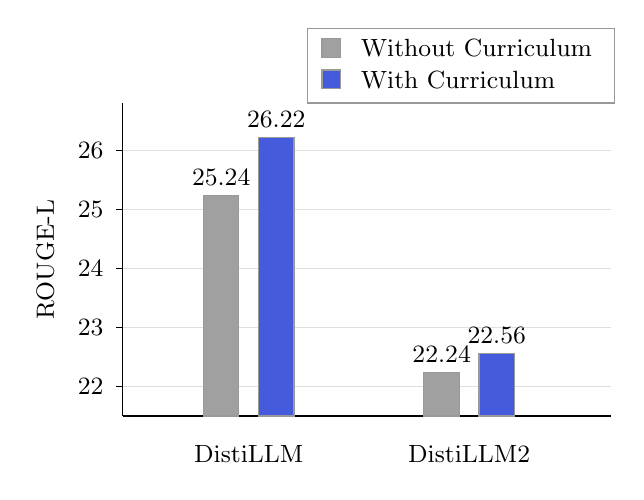
\begin{tikzpicture}[font=\small]

% --------------------
% Config
% --------------------
\def\ymin{21.5}
\def\ymax{26.8}
\def\yscale{0.75} % cm per ROUGE unit)

\def\barw{0.45}   % bar width
\def\gap{0.25}    % gap between bars within a group (smaller = closer)
\def\xA{1.6}      % center x of group 1
\def\xB{4.4}      % center x of group 2

\definecolor{cWithout}{RGB}{160,160,160}
\definecolor{cWith}{RGB}{70,90,220}

% --------------------
% Data
% --------------------
\def\aWithout{25.24}
\def\aWith{26.22}
\def\bWithout{22.24}
\def\bWith{22.56}

\pgfmathsetmacro{\Hmax}{(\ymax-\ymin)*\yscale}
\pgfmathsetmacro{\hAwithout}{(\aWithout-\ymin)*\yscale}
\pgfmathsetmacro{\hAwith}{(\aWith-\ymin)*\yscale}
\pgfmathsetmacro{\hBwithout}{(\bWithout-\ymin)*\yscale}
\pgfmathsetmacro{\hBwith}{(\bWith-\ymin)*\yscale}

% Group bar x positions
\pgfmathsetmacro{\xAleft}{\xA-(\barw+\gap/2)}
\pgfmathsetmacro{\xAright}{\xA+(\gap/2)}
\pgfmathsetmacro{\xBleft}{\xB-(\barw+\gap/2)}
\pgfmathsetmacro{\xBright}{\xB+(\gap/2)}

% Axis length in x
\def\xend{6.2}

% --------------------
% Axes
% --------------------
\draw[black] (0,0) -- (0,\Hmax);     % y-axis
\draw[black] (0,0) -- (\xend,0);     % x-axis

% Gridlines + y-ticks
\foreach \t in {22,23,24,25,26} {
  \pgfmathsetmacro{\yy}{(\t-\ymin)*\yscale}
  \draw[gray!25] (0,\yy) -- (\xend,\yy);
  \draw[black] (-0.08,\yy) -- (0,\yy);
  \node[anchor=east] at (-0.12,\yy) {\t};
}

% Y-axis label
\node[rotate=90, anchor=south] at (-0.75,0.5*\Hmax) {ROUGE-L};

% --------------------
% Bars: Group A (DistiLLM)
% --------------------
\draw[fill=cWithout, draw=black!40] (\xAleft,0) rectangle ++(\barw,\hAwithout);
\draw[fill=cWith,    draw=black!40] (\xAright,0) rectangle ++(\barw,\hAwith);

% Value labels
\node[anchor=south] at (\xAleft+0.5*\barw,\hAwithout) {\aWithout};
\node[anchor=south] at (\xAright+0.5*\barw,\hAwith) {\aWith};

% --------------------
% Bars: Group B (DistiLLM2)
% --------------------
\draw[fill=cWithout, draw=black!40] (\xBleft,0) rectangle ++(\barw,\hBwithout);
\draw[fill=cWith,    draw=black!40] (\xBright,0) rectangle ++(\barw,\hBwith);

% Value labels
\node[anchor=south] at (\xBleft+0.5*\barw,\hBwithout) {\bWithout};
\node[anchor=south] at (\xBright+0.5*\barw,\hBwith) {\bWith};

% --------------------
% X labels
% --------------------
\node[anchor=north] at (\xA, -0.25) {DistiLLM};
\node[anchor=north] at (\xB, -0.25) {DistiLLM2};
% --------------------
\begin{scope}[shift={(2.35,\Hmax-0.0)}]
  \draw[fill=white, draw=black!40] (0,0) rectangle (3.9,0.95);

  \draw[fill=cWithout, draw=black!40] (0.18,0.58) rectangle (0.42,0.82);
  \node[anchor=west] at (0.55,0.70) {Without Curriculum};

  \draw[fill=cWith, draw=black!40] (0.18,0.18) rectangle (0.42,0.42);
  \node[anchor=west] at (0.55,0.30) {With Curriculum};
\end{scope}

\end{tikzpicture}%
} % Ends the resizebox
\captionof{figure}{Comparison between curriculum-based and full-step distillation for hidden-state targets.}
\label{fig:curriculum_ablation}
\end{minipage}

\subsection{Direct Interpolation without a Learned Velocity Field}

To isolate the necessity of the learned velocity field $v_\theta$, we compare CONTRA-KD against a baseline that performs direct target interpolation without velocity field modeling. In this baseline, intermediate distillation targets are constructed via direct linear interpolation between student and teacher representations using the same curriculum schedule creating the target  $h_S + k (h_T - h_S)$.

\begin{table}[htbp]
  \centering
  \caption{Comparison with direct linear interpolation without velocity field (GPT2 1.5B $\rightarrow$ 0.1B with DistiLLM objective). ROUGE-L scores (\%) are averaged over 5 seeds $\pm$ standard deviation.}
  \label{tab:direct_interpolation}
  \resizebox{\linewidth}{!}{%
    \begin{tabular}{lcccccc}
      \toprule
      \textbf{Method} & \textbf{Dolly} & \textbf{Self-Inst} & \textbf{Vicuna} & \textbf{S-NI} & \textbf{UnNI} & \textbf{Avg.} \\
      \midrule
      With velocity field (Ours) & \textbf{26.22}$_{\pm 0.31}$ & \textbf{12.99}$_{\pm 0.53}$ & \textbf{17.41}$_{\pm 0.30}$ & \textbf{25.07}$_{\pm 0.21}$ & \textbf{26.85}$_{\pm 0.11}$ & \textbf{21.71}$_{\pm 0.14}$ \\
      Without velocity field     & 25.05$_{\pm 0.28}$          & 12.18$_{\pm 0.42}$          & 16.21$_{\pm 0.31}$          & 23.13$_{\pm 0.25}$          & 24.92$_{\pm 0.09}$          & 20.30$_{\pm 0.13}$          \\
      \bottomrule
    \end{tabular}%
  }
\end{table}

As detailed in Table~\ref{tab:direct_interpolation}, removing the learned velocity field leads to a consistent and substantial degradation in performance. This ablation validates a core premise of our framework: simply interpolating linearly between unaligned representations across high-dimensional feature spaces provides noisy, suboptimal supervision signals. Because the intermediate feature representations of LLMs form complex, highly non-linear manifolds, direct Euclidean interpolation fails to capture local curvature or feature dynamics. The learned velocity field $v_\theta$ acts as a continuous transport map via Rectified Flow, guiding student updates along an optimal trajectory and proving essential for effective feature alignment.

\section{Conclusion}
In this work, we presented CONTRA-KD, a knowledge distillation framework that models distillation as a continuous-time alignment problem. By treating teacher and student models as dynamical systems, we proved that minimizing trajectory discrepancy implicitly bounds the difference in their velocity fields. Building on this, we employ a rectified flow formulation with curriculum-based guidance to progressively transfer knowledge. Extensive experiments across multiple model pairs on instruction-following benchmarks demonstrate the effectiveness and compatibility of CONTRA-KD with reasonable computational overhead, highlighting the promising direction of flow-based and dynamical-system perspectives in knowledge distillation.

% This paper presents a methodological contribution to the field of machine learning, focusing on improving the efficiency and stability of knowledge distillation for large language models. By framing distillation through continuous-time dynamics and trajectory alignment, our work aims to facilitate the transfer of capabilities from large models to smaller, more computationally efficient ones. Such techniques can help reduce the computational and environmental costs associated with deploying large-scale models, potentially enabling broader access to advanced language technologies.

% While we have illustrated the capability of our work in language domain, we believe it can be applied in broader fields. We encourage future potential research to discuss the applications of this work across domains, such as multi-modal LLMs.

\subsection*{AI use statement}

In this work, we used generative AI tools solely for polishing the writing of the manuscript. We did not use generative AI tools to generate research ideas, design experiments, generate or analyze experimental results, or write any part of the theoretical proofs presented in this paper; all such tasks were performed entirely by the authors. All AI-assisted text was reviewed and edited by the authors to ensure accuracy and that it faithfully reflects our original contributions, methodology, and findings. We take responsibility for the final content of this work, including text, claims, and artifacts produced with the aid of generative AI.

\subsection*{Reproducibility statement}

We have taken several steps to facilitate reproducibility of our results. The complete derivation and proof of Theorem~\ref{def:inj}, which establishes the connection between trajectory alignment and velocity alignment, is provided in Appendix~\ref{app:proof}. The full training procedure for the velocity field and the two-phase CONTRA-KD distillation loop are given as pseudocode in Algorithm~\ref{alg:train_v_theta} and Algorithm~\ref{alg:contra_distillation} (Appendix~\ref{app:contra_algo}), respectively. Architectural details of the velocity field, including its embedding scheme, feed-forward block design, and per-model hidden dimension configuration, are described in Appendix~\ref{app:experiment} (Section~C.1), and all training hyperparameters, optimization settings, and hardware configuration are provided in Appendix~C.2. Dataset preprocessing and splits for \textit{databricks-dolly-15k} and the five evaluation benchmarks are described in Section~\ref{sec:exp_setup} and Appendix~C.2, and the LLM-as-a-judge evaluation protocol, including the exact prompt used, is given in Appendix~C.3 and Figure~\ref{fig:judge_prompt}. We will release our code as anonymous supplementary material to enable full reproduction of our experiments.


% \subsubsection*{Author Contributions}
% If you'd like to, you may include  a section for author contributions as is done
% in many journals. This is optional and at the discretion of the authors.

% \subsubsection*{Acknowledgments}
% Use unnumbered third level headings for the acknowledgments. All
% acknowledgments, including those to funding agencies, go at the end of the paper.


\bibliography{iclr2027_conference}
\bibliographystyle{iclr2027_conference}

\newpage
\appendix
\section{Related work}
\paragraph{Knowledge distillation of LLMs.} Knowledge Distillation (KD) \cite{hinton2015distillingknowledgeneuralnetwork} is a model compression technique where a student learns from a teacher model's outputs. A line of research has focused on treating distillation as a sequence-level alignment problem \cite{kim2016sequencelevelknowledgedistillation}. More recent methods have built on this, by using Kullback–Leibler divergence on student-generated outputs (SGOs) \cite{lin2020autoregressiveknowledgedistillationimitation}, employing Jensen-Shannon divergence \cite{agarwal2024onpolicydistillationlanguagemodels}, Reverse KLD \cite{gu2024minillmknowledgedistillationlarge, wu2024rethinkingkullbackleiblerdivergenceknowledge}, or skewed variants of KLD \cite{ko2024distillmstreamlineddistillationlarge, ko2025distillm2contrastiveapproachboosts}. Entropy-aware variants further adapt the choice of divergence per-token based on the teacher's local uncertainty \cite{Jin2026EntropyAwareOD}, and there is also growing interest in distilling through raw, unnormalized logits rather than softmax outputs \cite{kim2026distillationlargelanguagemodels}.

\paragraph{Intermediate representations distillation.} A complementary line of work distills a teacher's intermediate representations, motivated by the observation that deep models encode rich hierarchical information beyond their final outputs \cite{skean2025layerlayeruncoveringhidden}. Early successes along this direction were demonstrated for BERT-style architectures \cite{sanh2020distilbertdistilledversionbert, jiao2020tinybertdistillingbertnatural}. More recent methods have refined how this comparison is made rather than simply where: matching hidden states via Centered Kernel Alignment removes the requirement that student and teacher share a hidden dimension \cite{dasgupta2025improving}; a residual-learning objective instead trains the student to regress the difference between its own state and a projected teacher state, guarding against propagating the teacher's own mistakes \cite{on2026knowledge}. Inspired by interpreting Transformers as discretizations of Ordinary Differential Equations (ODEs) \cite{chen2019neuralordinarydifferentialequations, lu2019understandingimprovingtransformermultiparticle}, Feature Dynamic Distillation instead frames KD as aligning the trajectories of a coarse ODE solver (the student) with those of a fine-grained one (the teacher), matching both feature states and their first-order layer-to-layer differences \cite{gong-etal-2025-beyond}. While each of these approaches captures a different facet of the teacher's intermediate computation, all of them still compare states, residuals, or directions at a fixed set of layer checkpoints rather than the continuous path connecting them, which limits their ability to capture the global geometry of the teacher's feature flow.

\paragraph{Cross-tokenizer knowledge distillation.} Extending KD beyond teacher-student pairs that share a vocabulary, cross-tokenizer methods must additionally resolve a mismatch in sequence length and output dimensionality between the two models. ULD \cite{boizard2025crosstokenizerdistillationuniversallogit} applies a truncation strategy to align sequence lengths and logit dimensions, enabling direct comparison of output distributions. MinED \cite{Wan2024KnowledgeFO} instead relies on edit-distance-based token alignment to bridge mismatched tokenizations. Building on this line, MultiLevelOT \cite{cui2025multileveloptimaltransportuniversal} introduces an approximate Optimal Transport objective to reduce divergence at both the token and sequence level. DSKD \cite{zhang2024dualspaceknowledgedistillationlarge} projects student hidden states into the teacher's space and vice versa, and further introduces a cross-model attention mechanism that aligns tokens across tokenizers via embedding similarity. Rather than a static similarity-based alignment, contextual dynamical mapping \cite{Chen2025EnhancingCK} learns a context-conditioned correspondence between teacher and student tokens. Most recently, ALM \cite{minixhofer2025universalcrosstokenizerdistillationapproximate} refines token alignment further by exhaustively enumerating decoded chunks to identify equivalent segments between teacher and student outputs. Despite this progression, each approach carries its own limitation: truncation-based strategies such as ULD can discard information at alignment boundaries; edit-distance alignment as in MinED becomes brittle as vocabularies diverge further; optimal-transport objectives such as MultiLevelOT improve alignment quality but at a real computational cost; and exhaustive matching as in ALM scales poorly with vocabulary size and sequence length. We instead sidestep explicit token-level alignment altogether, identifying shared character-level boundaries via Longest Common Subsequence to construct token spans, and performing our trajectory-based distillation at the span level, where sequence lengths are guaranteed to match by construction.
\section{Theory Development}
In this section, we will give mathematical proof showing that by minimizing the continuous trajectory error, we implicitly constrain the student's governing vector field $v_S$ to align with the effective dynamics $v_T$ of the teacher. 

\begin{proof}
We start with    
\begin{align*}
\delta_{t} & =v_{S}\left(h_{T}\left(t\right),t\right)-v_{T}\left(h_{T}\left(t\right),t\right)\\
= & \left[v_{S}\left(h_{T}\left(t\right),t\right)-v_{S}\left(h_{S}\left(t\right),t\right)\right]\\
 & +\left[v_{S}\left(h_{S}\left(t\right),t\right)-v_{T}\left(h_{T}\left(t\right),t\right)\right].
\end{align*}

This leads to
\begin{align*}
\Vert\delta_{t}\Vert_{\mathcal{L}_{2}} & \leq\Vert v_{S}\left(h_{T}\left(t\right),t\right)-v_{S}\left(h_{S}\left(t\right),t\right)\Vert_{\mathcal{L}_{2}}\\
 & +\Vert v_{S}\left(h_{S}\left(t\right),t\right)-v_{T}\left(h_{T}\left(t\right),t\right)\Vert_{\mathcal{L}_{2}}\\
 & =\Vert v_{S}\left(h_{T}\left(t\right),t\right)-v_{S}\left(h_{S}\left(t\right),t\right)\Vert_{\mathcal{L}_{2}}\\
 & +\Vert\frac{d}{dt}\left[h_{S}\left(t\right)-h_{T}\left(t\right)\right]\Vert_{\mathcal{L}_{2}}.
\end{align*}

Using the $M$-Lipchitz, we have
\[
\Vert v_{S}\left(h_{T}\left(t\right),t\right)-v_{S}\left(h_{S}\left(t\right),t\right)\Vert_{\mathcal{L}_{2}}\leq M\Vert h_{T}\left(t\right)-h_{S}\left(t\right)\Vert_{\mathcal{L}_{2}}
\]

Finally, we reach the conclusion
\begin{align}
\Vert\delta_{t}\Vert_{\mathcal{L}_{2}} & \leq M\Vert h_{T}\left(t\right)-h_{S}\left(t\right)\Vert_{\mathcal{L}_{2}}\nonumber \\
 & +\Vert\frac{d}{dt}\left[h_{S}\left(t\right)-h_{T}\left(t\right)\right]\Vert_{\mathcal{L}_{2}}.\label{eq:delta_bound_new}
\end{align}
\end{proof}

\label{app:proof}

\section{Experimental Details}
\label{app:experiment}
\subsection{Velocity Field Design and Configurations}
For training as a neural network, we design the velocity field $v_{\theta}$ using components based on the design of Transformers \cite{vaswani2023attentionneed}. We use 2 embedding layers to encode the time step and layer step information, along with an input projection to project hidden states from the teacher model's dimension to a smaller internal dimension (called \textit{velocity field's hidden dimension}) to reduce the velocity field's hidden dimension size. The time and layer embeddings are then added to the projected input hidden states.

The embedded input goes through a sequence of feed-forward blocks, each constructed similar to the feed-forward network in a Transformer \cite{vaswani2023attentionneed} block. The representations first go through a layer normalization module \cite{ba2016layernormalization} to reduce variance, allowing the training process to be more stable. Then, they go through 2 linear layers with a GELU \cite{hendrycks2023gaussianerrorlinearunits} activation and the in-between dimension size of 4 times the model's hidden dimension size. Finally, the representation vectors go through a dropout module to ensure robustness of the network, before passing through an output projection back to the teacher's space.

In our experiments, to ensure consistency of CONTRA-KD's performance between pairs of teacher-student, which have different number of layers and hidden dimension sizes, we fix the number of layers (i.e., feed-forward blocks) of the velocity field model to 2 and the number of layers to distill between teacher and student to 4. Additionally, we set the model's hidden dimension size to 1024 for GPT2 models, 2400 for OpenLLaMA2 models, and 3200 for LLaMA2 models. The values are selected according to the teacher models' hidden dimension size (1600 for GPT2 1.5B, 3200 for OpenLLaMA2 7B, and 5120 for LLaMA2 13B), specifically around \textit{60\%} of the teachers' dimension size. This keeps the velocity fields compact while still allowing for effective distillation between larger models. We conduct additional ablation studies on hidden dimension size and number of layers of the velocity field in Appendix \ref{app:ablation}.

\subsection{Training Details}
Our experiments are based on previous implementation setups by \cite{gu2024minillmknowledgedistillationlarge, ko2024distillmstreamlineddistillationlarge,gong-etal-2025-beyond}. We use a preprocessed version of \textit{databricks-dolly-15k} provided by \cite{zhang2024dualspaceknowledgedistillationlarge}, consisting of around 11,500 samples for training, 1000 samples for validation, and 500 samples for testing. Along with that, we include a language modeling loss term on a randomly-sampled subset of 22,800 samples (i.e., about twice the size of Dolly training set) from the OpenWebText \cite{Gokaslan2019OpenWeb} corpus, as it has been shown by previous works to improve instruction-tuning performance. This loss term is only included in distillation experiments and not in SFT (teacher/student SFT and student warm-up) or velocity field training.

The models are trained using 1 NVIDIA H100 80GB GPU. Across all stages of our experiments, we use the same learning rate of 5e-4 and effective batch size of 16. For GPT2 models, we employ full fine-tuning for 20 epochs, except for the teacher GPT2 1.5B which is trained for only 10 epochs. For LLaMA2 and OpenLLaMA2 models, we fine-tune using LoRA \cite{hu2022lora} for 10 epochs with the rank and alpha both set at 16 and dropout rate at 0.1.

The student models are first fine-tuned for 3 epochs for warm-up on the training dataset. Then, they are used along with the corresponding teacher models for the initial training process of the velocity field for 3 epochs on the same dataset. The trained velocity fields act as initial checkpoints to be used for CONTRA-KD, where they are updated along with the student models to avoid distributional shifts.

Models are validated by evaluating their generated responses against the reference responses on the validation set using ROUGE-L \cite{lin-2004-rouge}. Responses are obtained using greedy sampling, and checkpoints with the best results are selected for later evaluation on benchmark datasets.

\subsection{Evaluation}
\paragraph{General Configurations.}
We sample responses from each model using temperature of 1.0, top\_p of 1.0, and max-length limit of 512.

\paragraph{LLM-as-a-judge.}
We use \texttt{GPT-4o-mini} as the judge, following prior work on LLM-based evaluation \cite{zheng2023judgingllmasajudgemtbenchchatbot}, for pairwise comparison of responses, comparing the baseline's response and CONTRA-KD's response for a given input prompt. For each baseline method and input prompt, we ask \texttt{GPT-4o-mini} to compare the responses between the student trained using the baseline method and the student trained using the same baseline with CONTRA loss term included, using the prompt format in Figure \ref{fig:judge_prompt} and setting the temperature of 0.7 for \texttt{GPT-4o-mini}. We record the number of baseline wins, CONTRA-KD wins, and ties for 3 benchmark datasets: Dolly, Self-Instruct, and Vicuna.

\paragraph{ROUGE-L.}
We sample responses using 5 random seeds $\{10, 20, 30, 40, 50\}$ and average results over the 5 seeds for each benchmark dataset: Dolly, Self-Instruct, Vicuna, Super-Natural Instructions, Unnatural Instructions.

\begin{figure}[htpb]
\centering
\fbox{
\begin{minipage}{0.95\linewidth}
\small
\textbf{[System]}\\
Please act as an impartial judge and compare the quality of response A and response B provided by two AI assistants to the user question displayed below. You should choose the assistant that follows the user's instructions and answers the user's question better.

Your evaluation should consider factors such as the helpfulness, relevance, accuracy, depth, creativity, and level of detail of their responses.

Avoid any position biases and ensure that the order in which the responses were presented does not influence your decision. Do not allow the length of the responses to influence your evaluation. Do not favor certain names of the assistants. Be as objective as possible.

Output your final verdict by strictly following this format:\\
If A is significantly better overall, answer ``A''.\\
If B is significantly better overall, answer ``B''.\\
If both are similar in quality (both bad or both good or not significantly different), answer ``Tied''.

\medskip
\textbf{[Question]}\\
\texttt{\{question\}}

\medskip
\textbf{[Response A]}\\
\texttt{\{response\_A\}}\\
\textbf{[End of Response A]}

\medskip
\textbf{[Response B]}\\
\texttt{\{response\_B\}}\\
\textbf{[End of Response B]}
\end{minipage}
}
\caption{Prompt used for pairwise response quality evaluation.}
\label{fig:judge_prompt}
\end{figure}

\begin{algorithm}[t]
  \caption{CONTRA-KD Distillation}
  \label{alg:contra_distillation}
  \begin{algorithmic}[1]
    \STATE \textbf{Input:} student $q_{\phi_0}$ with parameters $\phi_0$, teacher $p$, pre-trained velocity field $v_\theta$ and projector $f_{\text{proj}}$, data $\mathcal{D}$, layer maps $I^S, I^T$
    \STATE \textbf{Output:} Student model $q_{\phi_E}$ with trained parameters $\phi_E$
    
    \FOR{epoch $e = 1,2,...,E$}
    \STATE $k \gets \frac{e}{E}$
    \FOR{each batch $\{x_i\}$ in $\mathcal{D}$}

      \STATE \textcolor{gray}{// --- Phase 1: Update Student Model ---}
      \STATE Initialize $\mathcal{L}_{CONTRA} \gets 0$

      \FOR{$j = 1,2,...,L_D$}
        \STATE $h_S^j \gets f_{\text{proj}}\!\left(q_{\phi_{e-1}}(\{x_i\}, \text{layer}=l_j^S)\right)$ 
        \STATE $\tilde{h}_S^j \gets h_S^j + k \cdot v_\theta(h_S^j, t=0, j)$
        \STATE $\mathcal{L}_{\text{CONTRA}} \gets \mathcal{L}_{\text{CONTRA}} + D_{\text{cos}}(h_S^j, \tilde{h}_S^j)$
      \ENDFOR
      \STATE Compute $\mathcal{L}_{KD}$ using $p(x_i)$ and $q_{\phi_{e-1}}(x_i)$
      \STATE $\mathcal{L}_{Total} \gets \mathcal{L}_{CE} + \mathcal{L}_{KD} + \mathcal{L}_{CONTRA}$
      \STATE Update $\phi_{e} \gets \phi_{e-1} - \eta \nabla_\phi \mathcal{L}_{Total}$

    \ENDFOR
    \STATE \textcolor{gray}{// --- Phase 2: Adapt Velocity Field \& Projector ---}
    \STATE Update velocity field $v_\theta$ and projector $f_{\text{proj}}$ based on Algorithm~\ref{alg:train_v_theta} using teacher $p$, student $q_{\phi_{e}}$, data $\mathcal{D}$, layer maps $I_S, I_T$
    \ENDFOR
    \STATE \textbf{return} $q_{\phi_{E}}$
  \end{algorithmic}
\end{algorithm}

\section{Detailed Algorithm}
\label{app:contra_algo}

Algorithm~\ref{alg:contra_distillation} details the full two-phase training loop introduced in Section~\ref{sec:distill}: Phase 1 updates the student parameters $\phi$ using the combined loss $\mathcal{L}_{Total}$, and Phase 2 re-adapts the velocity field $v_\theta$ and projector $f_{\text{proj}}$ on the updated student following Algorithm~\ref{alg:train_v_theta}, preventing distributional drift between the student and the flow it is being aligned to.


\section{Additional Experimental Results.}
\subsection{Additional Results of Larger Teacher--Student Pair}
\label{app:large_scale}
To demonstrate scalability to larger models, we conduct additional experiments on LLaMA2~\cite{touvron2023llamaopenefficientfoundation} with a 13B teacher and 7B student. ROUGE-L scores and GPT-4o-mini win/tie/loss rates are reported in Tables~\ref{app:winrates} and~\ref{app:results}, respectively.

CONTRA-KD consistently improves all baselines on this larger pair. In terms of ROUGE-L, average gains range from \textbf{+0.29\%} (DistiLLM) to \textbf{+0.64\%} (FDD), with DistiLLM-2 + CONTRA achieving the highest average score of \textbf{30.71}. Most notably, DistiLLM-2 + CONTRA reaches a ROUGE-L score of \textbf{38.59} on the UnNI benchmark, substantially surpassing the teacher itself at 34.25, suggesting that our contrastive objective helps the student better generalize on unseen natural instructions at scale. GPT-4o-mini evaluations corroborate these gains, with CONTRA-KD winning more often than the baseline across all methods and datasets.

\begin{table*}[t]
\centering
\caption{Win / Tie / Loss rates (\%) of LLaMA2 on different benchmark datasets, evaluated by \texttt{GPT-4o-mini}.
\textbf{Win} indicates preference for the model trained with \textsc{CONTRA-KD} over the baseline (Ours Win),
\textbf{Loss} indicates preference for the baseline (Baseline Win), and \textbf{Tie} denotes equal quality.}
\label{app:winrates}

\resizebox{\textwidth}{!}{%
\begin{tabular}{l ccc ccc ccc}
\toprule
& \multicolumn{9}{c}{\textbf{Evaluation Set}} \\
\cmidrule(lr){2-10}
\textbf{Method}
& \multicolumn{3}{c}{\textit{Dolly}}
& \multicolumn{3}{c}{\textit{Self-Instruct}}
& \multicolumn{3}{c}{\textit{Vicuna}} \\
\cmidrule(lr){2-4} \cmidrule(lr){5-7} \cmidrule(lr){8-10}
& Win & Tie & Loss
& Win & Tie & Loss
& Win & Tie & Loss \\
\midrule

\multicolumn{10}{c}{\textit{LLaMA2 13B $\rightarrow$ 7B}} \\
\midrule

FDD (+CONTRA vs.\ baseline)
& \textbf{44.00} & 19.60 & 36.40
& 38.43 & 23.14 & 38.43
& \textbf{48.75} & 10.00 & 41.25 \\

DistiLLM (+CONTRA vs.\ baseline)
& \textbf{41.20} & 22.60 & 36.20
& \textbf{43.80} & 14.40 & 41.80
& \textbf{46.25} & 15.00 & 38.75 \\

DistiLLM-2 (+CONTRA vs.\ baseline)
& \textbf{40.40} & 26.60 & 33.00
& \textbf{43.80} & 15.29 & 40.91
& \textbf{45.00} & 21.25 & 33.75 \\

\bottomrule
\end{tabular}
}
\end{table*}

\begin{table}[htbp]
\centering
\small
\setlength{\tabcolsep}{4.5pt}
\caption{Effects of CONTRA-KD on SOTA methods for LLaMA2. ROUGE-L scores (\%) averaged over 5 random seeds $\pm$ standard deviation.}
\label{app:results}
\begin{tabular}{lcccccc}
\toprule
\textbf{Method} & \textbf{Dolly} & \textbf{Self-Inst} & \textbf{Vicuna} & \textbf{S-NI} & \textbf{UnNI} & \textbf{Avg.} \\
\midrule
\multicolumn{7}{c}{\textit{LLaMA2 13B $\rightarrow$ 7B}} \\
\midrule
Teacher    & 30.19 & 23.92 & 19.56 & 34.53 & 34.25 & 28.49 \\
SFT        & 28.38 & 20.32 & 17.72 & 34.37 & 33.25 & 26.81 \\
\midrule
DistiLLM   & 31.10$_{\pm 0.57}$ & 23.22$_{\pm 0.43}$ & 21.38$_{\pm 0.35}$ & \textbf{36.30}$_{\pm 0.34}$ & 37.03$_{\pm 0.07}$ & 29.81$_{\pm 0.17}$ \\
\textit{+CONTRA}
           & \textbf{31.45}$_{\pm 0.20}$ & \textbf{23.69}$_{\pm 0.52}$ & \textbf{21.48}$_{\pm 0.14}$ & 36.19$_{\pm 0.26}$ & \textbf{37.70}$_{\pm 0.15}$ & \textbf{30.10}$_{\pm 0.13}$ \\
\midrule
FDD        & 30.59$_{\pm 0.44}$ & 22.12$_{\pm 0.52}$ & 20.87$_{\pm 0.29}$ & 35.91$_{\pm 0.33}$ & 36.48$_{\pm 0.13}$ & 29.19$_{\pm 0.16}$ \\
\textit{+CONTRA}
           & \textbf{31.55}$_{\pm 0.27}$ & \textbf{22.80}$_{\pm 1.02}$ & \textbf{20.92}$_{\pm 0.15}$ & \textbf{36.81}$_{\pm 0.17}$ & \textbf{37.08}$_{\pm 0.13}$ & \textbf{29.83}$_{\pm 0.22}$ \\
\midrule
DistiLLM-2 & 31.76$_{\pm 0.32}$ & \textbf{24.49}$_{\pm 0.25}$ & 21.96$_{\pm 0.38}$ & 35.98$_{\pm 0.24}$ & 36.57$_{\pm 0.08}$ & 30.15$_{\pm 0.12}$ \\
\textit{+CONTRA}
           & \textbf{32.19}$_{\pm 0.57}$ & 23.97$_{\pm 0.49}$ & \textbf{22.27}$_{\pm 0.26}$ & \textbf{36.52}$_{\pm 0.30}$ & \textbf{38.59}$_{\pm 0.05}$ & \textbf{30.71}$_{\pm 0.17}$ \\
\bottomrule
\end{tabular}
\end{table}

% \begin{minipage}[t]{0.48\textwidth}
% % \begin{table}[t]
% \vspace{0pt} % Top anchor
% \centering
% % Table captions traditionally go ABOVE the table
% \captionof{table}{Training cost analysis for LLaMA2. We report the average wall-clock time per epoch in minutes.}
% \label{tab:training_time_llama}
% \vspace{0.5em} % Adds a tiny gap between caption and table
% \begin{small}
% % Changed \linewidth to 0.85\linewidth to shrink the table
% \resizebox{0.85\linewidth}{!}{%
% \begin{tabular}{lccc}
% \toprule
% \textbf{Method} & \textbf{Standard} & \textbf{+CONTRA} & \textbf{Increase} \\
% \midrule
% \multicolumn{4}{c}{\textit{LLaMA2 13B $\rightarrow$ 7B}} \\
% \midrule
% DistiLLM & 32.50 & 43.10 & 1.33$\times$ \\
% FDD      & 27.20 & 39.80 & 1.46$\times$ \\
% DistiLLM2 & 71.60 & 89.30 & 1.25$\times$ \\
% \bottomrule
% \end{tabular}%
% } % Ends the resizebox
% \end{small}
% \end{minipage}
% % \end{table}

% \subsection{Cross-tokenizer KD Results}
% \label{app:ctkd}
% \paragraph{Method.} To demonstrate the applicability of CONTRA-KD in cross-architecture, cross-tokenizer scenarios, we developed a simple adaptation by aligning sequence lengths between the teacher and the student models through the concept of token spans. While different models tokenize an input sequence differently, they tend to divide a word into multiple tokens. Therefore, we align the different token sequence lengths by identifying consecutive tokens (called a "token span") that contain the same sequence of characters in both input sequences. We identify corresponding pairs of token spans via Longest Common Subsequence (LCS), utilizing the character offsets of tokens to find matched segments of the input that correspond to the same piece of text. 

% By converting the sequence of tokens into a sequence of token spans, the length mismatch issue is resolved. To apply CONTRA-KD to this formed sequence, we construct a span representation by taking the average of the representations of the tokens within the span. We then distill using the rectified flow from the span representation of the student to the corresponding span representation of the teacher, effectively treating the models as if they shared a tokenizer and vocabulary. We also incorporate a divergence loss term to distill the span sequence at the logit-level, employing the Skew Reverse KL Divergence used by DistiLLM.

% \paragraph{Settings.} 

% \paragraph{Results.} Our experimental results, presented in Table \ref{tab:ctkd_results}, demonstrate that CONTRA-KD consistently outperforms other baselines on the majority of datasets under this simple adaptation to the cross-tokenizer scenario.

\subsection{Human Evaluation on Instruction-Following}
\label{sec:appendix_human_eval}

To complement our automated evaluation metrics and validate the reliability of our GPT-4o-mini judge, we conducted a blind human evaluation on a randomized subset of 100 instruction-following outputs from the \textit{Dolly} test set, comparing CONTRA-KD against the competitive CSD baseline. Each item was independently evaluated by three human annotators in a double-blind A/B testing setup.

\begin{table}[htbp]
\centering
\small
\setlength{\tabcolsep}{14pt}
\caption{Human-evaluated Win / Tie / Loss rates (\%) for CONTRA-KD versus the CSD baseline on 100 \textit{Dolly} test samples across three independent annotators and pooled judgment.}
\label{tab:human_eval}
\begin{tabular}{lccc}
\toprule
\textbf{Evaluator} & \textbf{Win (\%)} & \textbf{Tie (\%)} & \textbf{Loss (\%)} \\
\midrule
Annotator 1 & \textbf{36.0} & 32.0 & 32.0 \\
Annotator 2 & \textbf{43.0} & 20.0 & 37.0 \\
Annotator 3 & \textbf{46.0} & 29.0 & 25.0 \\
\midrule
\textbf{Pooled} & \textbf{41.7} & 27.0 & 31.3 \\
\bottomrule
\end{tabular}
\end{table}

As presented in Table~\ref{tab:human_eval}, pooled human judgments preferred CONTRA-KD in \textbf{41.7\%} of cases, compared to \textbf{31.3\%} for the baseline (with 27.0\% ties). When excluding ties, CONTRA-KD achieved a \textbf{57.1\% preference win rate}. These findings strongly mirror our GPT-4o-mini LLM-as-a-Judge evaluation, reinforcing that continuous trajectory alignment leads to tangibly higher generation quality and better instruction compliance.

\paragraph{Agreement Analysis.} To assess evaluation consistency, we measured both internal inter-annotator reliability and external alignment with the GPT-4o-mini judge. Pairwise agreement between individual human annotators and the LLM judge averaged 48.7\%. Inter-annotator agreement, measured via Fleiss' $\kappa$, showed slight agreement consistent with expected variance in open-ended response comparison. Crucially, both human majority vote and the automated LLM judge demonstrate identical directional preferences (favoring CONTRA-KD), validating the credibility of our automated evaluation pipeline.

\paragraph{Human Evaluation Rubric.} Human annotators were provided with the interface instructions and evaluation prompt shown in Figure~\ref{fig:human_eval_prompt}.

\begin{figure}[htpb]
\centering
\fbox{
\begin{minipage}{0.95\linewidth}
\small
\textbf{[Instructions for Annotators]}\\
Please act as an impartial judge and compare the quality of Response A and Response B provided by two AI assistants to the user question displayed for each item below. You should choose the assistant that follows the user's instructions and answers the question better.

Your evaluation should consider factors such as the helpfulness, relevance, accuracy, depth, creativity, and level of detail of their responses.

Avoid any position biases and ensure that the order in which the responses were presented does not influence your decision. Do not allow the length of the responses to influence your evaluation. Be as objective as possible.

Choose your verdict by strictly following this format:\\
If A is significantly better overall, select ``A''.\\
If B is significantly better overall, select ``B''.\\
If both are similar in quality (both bad, both good, or not significantly different), select ``Tied''.

\medskip
\textbf{[User Question]}\\
\texttt{\{question\}}

\medskip
\textbf{[Response A]}\\
\texttt{\{response\_A\}}

\medskip
\textbf{[Response B]}\\
\texttt{\{response\_B\}}
\end{minipage}
}
\caption{Instruction guidelines and prompt format provided to human annotators for pairwise evaluation.}
\label{fig:human_eval_prompt}
\end{figure}


\subsection{CONTRA as a Standalone Objective}
To isolate the exact contribution of our continuous trajectory alignment objective ($\mathcal{L}_{\text{CONTRA}}$), we evaluate a standalone version of our framework--\textbf{CONTRA only}--where the student is trained using solely cross-entropy and feature trajectory alignment ($\mathcal{L}_{\text{CE}} + \lambda \mathcal{L}_{\text{CONTRA}}$), omitting any output logit matching objective (e.g., DistiLLM or reverse KL). Table~\ref{tab:contra_standalone} compares \textbf{CONTRA only} against standard baseline approaches in their native configurations on the GPT-2 $1.5\text{B} \to 0.1\text{B}$ model pair across five benchmark datasets.

\begin{table}[htbp]
\centering
\small
\setlength{\tabcolsep}{4.5pt}
\caption{Standalone performance comparison of CONTRA-KD against baseline distillation objectives on GPT-2 $1.5\text{B} \to 0.1\text{B}$ using ROUGE-L scores.}
\label{tab:contra_standalone}
\begin{tabular}{lcccccc}
\toprule
\textbf{Method} & \textbf{Dolly} & \textbf{Self-Inst} & \textbf{Vicuna} & \textbf{S-NI} & \textbf{UnNI} & \textbf{Avg.} \\
\midrule
% SFT & 23.33 & 10.56 & 15.12 & 17.08 & 20.07 & 17.23 \\
FDD                   & 24.27$_{\pm 0.19}$ & 11.23$_{\pm 0.28}$ & 14.69$_{\pm 0.40}$ & 19.65$_{\pm 0.20}$ & 22.50$_{\pm 0.18}$ & 18.47$_{\pm 0.12}$ \\
CSD                   & 24.28$_{\pm 0.32}$ & 10.76$_{\pm 0.55}$ & 15.95$_{\pm 0.34}$ & 20.01$_{\pm 0.30}$ & 22.32$_{\pm 0.19}$ & 18.66$_{\pm 0.16}$ \\
DistiLLM              & \textbf{25.17}$_{\pm 0.36}$ & \textbf{11.93}$_{\pm 0.18}$ & 16.63$_{\pm 0.26}$ & \textbf{23.29}$_{\pm 0.27}$ & \textbf{25.41}$_{\pm 0.16}$ & \textbf{20.49}$_{\pm 0.11}$ \\
DistiLLM-2            & 22.22$_{\pm 0.09}$ & 11.13$_{\pm 0.67}$ & \textbf{17.19}$_{\pm 0.07}$ & 21.58$_{\pm 0.37}$ & 24.39$_{\pm 0.20}$ & 19.30$_{\pm 0.17}$ \\
\midrule
\textbf{CONTRA only (Ours)} & 24.53$_{\pm 0.28}$ & 11.76$_{\pm 0.28}$ & 15.67$_{\pm 0.32}$ & 19.70$_{\pm 0.22}$ & 23.11$_{\pm 0.10}$ & 18.95$_{\pm 0.11}$ \\
\bottomrule
\end{tabular}
\end{table}

Operating purely on internal representations, \textbf{CONTRA only} achieves an average score of $18.95$, outperforming both Feature Dynamics Distillation (FDD, $18.47$) and Concrete Score Matching (CSD, $18.66$). This validates that aligning continuous Rectified Flow trajectories provides superior feature-level transfer compared to matching discrete, local derivatives.

Feature-level alignment ensures that student hidden states follow mathematically smooth, teacher-directed ODE paths through depth, while logit-level objectives sharpen the final output probability distribution over the vocabulary. Combining both mechanisms (Ours + DistiLLM) yields the highest performance across all benchmarks.

\subsection{Comparisons Against Baselines with Matched Computation}

To ensure that the performance gains observed with \textit{+CONTRA} are not merely an artifact of the additional training stage, it is crucial to isolate the effect of training duration. We conduct additional experiments where models are trained using baseline methods with more training steps. Specifically, we increase the number of epochs by 50\% to assess whether using baseline methods with a longer training time can match or outperform our method. We run experiments on two pairs of teacher-student models (GPT-2 1.5B $\rightarrow$ 0.1B and OpenLLaMA-2 7B $\rightarrow$ 3B) and for three baselines (SFT, Vanilla KD, DistiLLM); the results (ROUGE-L score, averaged over 5 random seeds) are summarized in Table \ref{tab:extended_training_ablation}. As shown by the results, training baselines longer does not yield better performance than CONTRA; it even leads to worse results. This is most likely due to overfitting, as models are exposed to the training dataset more, whereas CONTRA-KD 'extracts' more information from a training step rather than making the model view the dataset more times.

\begin{table}[htbp]
\centering
\small
\caption{Ablation study on training duration. +CONTRA maintains superior performance across all evaluation datasets without relying solely on increased training duration.}
\label{tab:extended_training_ablation}
\vspace{0.5em}
\begin{tabular}{lccccc}
\toprule
\textbf{Method} & \textbf{Dolly} & \textbf{Self-Inst} & \textbf{Vicuna} & \textbf{S-Inst} & \textbf{Avg.} \\
\midrule
\multicolumn{6}{c}{\textbf{GPT-2 (1.5B $\rightarrow$ 0.1B)}} \\
\midrule
SFT & 23.33 & 10.56 & 15.12 & 17.08 & 16.52 \\
SFT (longer) & 23.29 & 8.81 & 14.67 & 15.46 & 15.56 \\
KD & 23.52 & 11.23 & 15.92 & 20.68 & 17.84 \\
KD (longer) & 23.37 & 10.60 & 15.36 & 19.42 & 17.19 \\
DistiLLM & 25.17 & 11.93 & 16.63 & 23.29 & 19.26 \\
DistiLLM (longer) & 24.86 & 11.52 & 16.79 & 20.26 & 18.36 \\
\midrule
DistiLLM + CONTRA (Ours) & \textbf{26.22} & \textbf{12.99} & \textbf{17.41} & \textbf{25.07} & \textbf{20.42} \\
\midrule
\multicolumn{6}{c}{\textbf{OpenLLaMA-2 (7B $\rightarrow$ 3B)}} \\
\midrule
SFT & 24.95 & 17.38 & 14.58 & 28.65 & 21.39 \\
SFT (longer) & 24.29 & 16.48 & 17.03 & 28.37 & 21.54 \\
KD & 25.10 & 17.11 & 16.64 & 28.93 & 21.95 \\
KD (longer) & 21.75 & 15.47 & 16.14 & 25.90 & 19.82 \\
DistiLLM & 28.97 & 19.39 & 19.60 & 34.46 & 25.61 \\
DistiLLM (longer) & 28.37 & 19.53 & 19.52 & 34.24 & 25.42 \\
\midrule
DistiLLM + CONTRA (Ours) & \textbf{29.04} & \textbf{20.20} & \textbf{19.66} & \textbf{35.65} & \textbf{26.14} \\
\bottomrule
\end{tabular}
\end{table}



\section{Additional Analysis}
\label{app:ablation}
\subsection{Non-linear Interpolant Path Analysis} 
A core efficiency mechanism of CONTRA-KD is the generation of the dynamic distillation target via an explicit Euler update along a learned flow (see Section \ref{sec:distill}). This approximation is geometrically faithful when the underlying flow trajectory is linear, but may incur truncation error when applied to curved paths. To validate this design choice, we compare our linear Rectified Flow against two non-linear path formulations commonly used in diffusion models: Variance Preserving (VP) ODE \cite{song2021scorebasedgenerativemodelingstochastic} and Variance Exploding (VE) ODE \cite{song2021scorebasedgenerativemodelingstochastic}.

The flow trajectories are defined by a generalized interpolant $H_t$ between the student state $h_S^{j}[i]$ and teacher state $h_T^{j}[i]$:
\begin{equation}
    H_t = \sigma_t h_S^{j}[i] + \alpha_t h_T^{j}[i]
\end{equation}
where $\sigma_t$ and $\alpha_t$ control the mixing schedule. We compare three schedules:
\begin{itemize}
    \item \textbf{Rectified Flow (Ours):} The linear path with $\alpha_t = t$ and $\sigma_t = 1-t$.
    \item \textbf{VP ODE:} A cosine-based schedule defined by $\alpha_t = \exp(-\frac{1}{4}a(1-t)^2 - \frac{1}{2}b(1-t))$ and $\sigma_t = \sqrt{1-\alpha_t^2}$, with $a=19.9$ and $b=0.1$.
    \item \textbf{VE ODE:} A geometric variance schedule defined by $\alpha_t = a(\frac{b}{a})^t$ and $\sigma_t = 1$, with $a=0.02$ and $b=100$.
\end{itemize}



\begin{minipage}[t]{0.55\textwidth}
\vspace{0pt}
The results in Table \ref{tab:path_ablation} show that the VP-ODE path causes a noticeable performance drop ($-0.53$ ROUGE-L). This indicates that curved interpolation paths are ill-suited for Euler-based target generation, as local curvature introduces truncation error even when using partial steps along the flow. While VE-ODE performs comparably to the linear baseline, it requires careful hyperparameter tuning ($a, b$) and offers no performance gain. In contrast, the linear Rectified Flow consistently provides a stable and accurate approximation under Euler updates, making it the most effective choice for curriculum-based trajectory distillation.
\end{minipage}% 
\hfill
\begin{minipage}[t]{0.4\textwidth}
\vspace{0pt} 
\vspace{-\intextsep} % Pulls the table up to cancel the default [H] padding
\begin{table}[H]
\centering
\caption{Ablation study on the impact of interpolation path geometry (GPT-2 1.5B $\to$ 0.1B) in DistiLLM.}
\label{tab:path_ablation}
\begin{tabular}{lc}
\toprule
\textbf{Interpolation Path} & \textbf{ROUGE-L} \\
\midrule
Rectified Flow (Ours) & \textbf{26.22} \\
VP-ODE & 24.71 \\
VE-ODE & 25.23 \\
\bottomrule
\end{tabular}
\end{table}
\end{minipage}

\subsection{Computational and Memory Cost}
\label{sec:projector_lmhead_impact}
We analyze the computational overhead introduced by adding CONTRA-KD by comparing the average wall-clock training time per epoch and peak memory usage across different distillation settings in Table \ref{tab:time_memory}. Incorporating CONTRA-KD leads to a moderate and consistent increase in training time, with the relative overhead remaining below $1.5\times$ in all configurations. In terms of memory usage, CONTRA-KD introduces minimal increase with only around 2\% for the GPT2 pair and moderate increase for the OpenLLaMA2 pair; the only exception is OpenLLaMA2 with the DistiLLM2 baseline, where the method uses a forward batch size doubled that of other baselines, which, combined with a larger velocity field, results in a higher memory overhead; the increase is still moderate given the baseline's high usage.

Overall, these results show that while CONTRA-KD introduces a manageable increase in training cost and memory usage, the overhead remains controlled across scales and methods, supporting its practicality for large-scale distillation settings.

\begin{table}[h]
\centering
\small
\caption{Average wall-clock time per epoch (minutes) and peak GPU memory usage (GB), for baseline methods and with CONTRA-KD incorporated.}
\label{tab:time_memory}
\vspace{0.5em}
\begin{tabular}{lccc ccc}
\toprule
& \multicolumn{3}{c}{\textbf{Time (min)}} & \multicolumn{3}{c}{\textbf{Memory (GB)}} \\
\cmidrule(lr){2-4} \cmidrule(lr){5-7}
\textbf{Method} & Std. & +CONTRA & Incr. & Std. & +CONTRA & Incr. \\
\midrule
\multicolumn{7}{c}{\textit{GPT2 1.5B $\rightarrow$ 0.1B}} \\
\midrule
DistiLLM  & 13.50 & 14.15 & 1.05$\times$ & 29.99 & 30.55 & 1.87\% \\
FDD       & 9.25  & 12.45 & 1.35$\times$ & 35.55 & 36.34 & 2.22\% \\
DistiLLM2 & 12.20 & 13.05 & 1.07$\times$ & 53.51 & 54.72 & 2.26\% \\
\midrule
\multicolumn{7}{c}{\textit{OpenLLaMA2 7B $\rightarrow$ 3B}} \\
\midrule
DistiLLM  & 28.50 & 32.90 & 1.15$\times$ & 41.35 & 43.05 & 4.11\% \\
FDD       & 23.80 & 26.90 & 1.13$\times$ & 53.64 & 57.29 & 6.80\% \\
DistiLLM2 & 65.90 & 78.60 & 1.19$\times$ & 52.84 & 67.36 & 27.48\% \\
\bottomrule
\end{tabular}
\end{table}

\subsection{Comparison with Ordinary Feature KD and Curriculum Decoupling}
\label{sec:ablation_feature_kd}

To position CONTRA-KD against standard intermediate feature distillation techniques, we clarify that conventional feature KD variants--specifically hidden-state Mean Squared Error and feature delta matching (matching first-order derivatives)--constitute the core formulation of Feature Dynamics Distillation (FDD)~\citep{gong-etal-2025-beyond}. Consequently, comparisons against FDD directly evaluate our framework against these ordinary feature KD objectives.

To further isolate the individual contributions of our continuous flow formulation from the progressive curriculum strategy, we evaluate four distinct configurations on the GPT-2 (1.5B $\rightarrow$ 0.1B) teacher--student pair: (i)~\textbf{FDD} (standard baseline combining state MSE and first-order delta losses), (ii)~\textbf{FDD + Curriculum} (applying our progressive step-size schedule directly to FDD targets), (iii)~\textbf{CONTRA only} (our continuous flow objective without FDD losses), and (iv)~\textbf{Ours + FDD} (the full combined framework).

\begin{table}[htbp]
\centering
\small
\setlength{\tabcolsep}{4.5pt}
\caption{Comparison of ordinary feature KD variants, curriculum scheduling, and standalone CONTRA (GPT-2 1.5B $\rightarrow$ 0.1B). ROUGE-L scores (\%) are averaged over 5 random seeds $\pm$ standard deviation.}
\label{tab:feature_kd_ablation}
\begin{tabular}{lcccccc}
\toprule
\textbf{Method} & \textbf{Dolly} & \textbf{Self-Inst} & \textbf{Vicuna} & \textbf{S-NI} & \textbf{UnNI} & \textbf{Avg.} \\
\midrule
FDD              & 24.27$_{\pm 0.19}$          & 11.23$_{\pm 0.28}$          & 14.69$_{\pm 0.40}$          & 19.65$_{\pm 0.20}$          & 22.50$_{\pm 0.18}$          & 18.47$_{\pm 0.12}$ \\
FDD + Curriculum & 23.37$_{\pm 0.59}$          & 10.77$_{\pm 0.30}$          & 14.80$_{\pm 0.23}$          & \textbf{21.62}$_{\pm 0.25}$ & 22.82$_{\pm 0.10}$          & 18.68$_{\pm 0.15}$ \\
CONTRA only      & 24.53$_{\pm 0.28}$          & \textbf{11.76}$_{\pm 0.28}$ & 15.67$_{\pm 0.32}$          & 19.70$_{\pm 0.22}$          & \textbf{23.11}$_{\pm 0.10}$ & 18.95$_{\pm 0.11}$ \\
\midrule
Ours + FDD       & \textbf{25.12}$_{\pm 0.43}$ & 11.46$_{\pm 0.38}$          & \textbf{16.05}$_{\pm 0.29}$ & 20.21$_{\pm 0.22}$          & 22.79$_{\pm 0.07}$          & \textbf{19.13}$_{\pm 0.14}$ \\
\bottomrule
\end{tabular}
\end{table}

As reported in Table~\ref{tab:feature_kd_ablation}, \textbf{CONTRA only} consistently outperforms standard \textbf{FDD}. This validates that parameterizing a continuous velocity field $v_\theta$ via Rectified Flow provides superior trajectory guidance compared to matching static intermediate states and discrete layer differences.

Furthermore, applying the progressive curriculum directly to FDD (\textbf{FDD + Curriculum}) leads to optimization instability and noticeable degradation on benchmarks such as \textit{Dolly} and \textit{Self-Instruct}. We attribute this to a fundamental geometric mismatch: FDD relies on localized, pointwise feature MSE and first-order difference vectors, which become uninformative or noisy when extrapolated across larger step distances required by long-range curriculum supervision. In contrast, CONTRA-KD explicitly models continuous vector fields across the representation space, ensuring well-conditioned supervision targets throughout all stages of curriculum scaling. Finally, combining continuous trajectory alignment with FDD (\textbf{Ours + FDD}) achieves the highest overall performance, demonstrating the complementary nature of continuous flow matching with traditional feature regularization.

\subsection{Alternative Cross-tokenizer Alignment via Edit Distance}
\label{app:edit_distance_alignment}

To complement the LCS-based span construction, we describe an alternative cross-tokenizer alignment strategy based on token-level edit distance. It operates on the same character-offset representation and produces the identical span-pair format, allowing the span-level rectified-flow objective and curriculum distillation to apply unchanged.

\paragraph{Span Construction via Edit Distance.}
As in the LCS variant, the teacher and student tokenize the same input $x$ but produce sequences of different lengths. Each token is annotated with its character-level span $(\mathrm{start}, \mathrm{end})$, yielding offset sequences $\mathbf{o}^T$ and $\mathbf{o}^S$. Special tokens with end offset $0$ and prompt tokens preceding the response start indices $s_i, s_j$ are excluded from alignment.

Let $\{a_i\}_{i=1}^{m}$ and $\{b_j\}_{j=1}^{n}$ denote the filtered student and teacher offset spans in the response region. We compute a Levenshtein alignment between the two span sequences, where two tokens match if and only if their character spans are identical. The dynamic-programming cost matrix $D[i][j]$ is initialized as $D[0][j]=j$, $D[i][0]=i$ and updated as:
\begin{equation}
    D[i][j] = \min \begin{cases}
        D[i-1][j-1] + \mathbb{I}[a_i \neq b_j] & \text{(substitute / match)} \\
        D[i-1][j] + 1 & \text{(delete)} \\
        D[i][j-1] + 1 & \text{(insert)}
    \end{cases}
\end{equation}
where $\mathbb{I}[\cdot]$ evaluates to $0$ if the two offset spans are identical and $1$ otherwise. Backtracking from $(m,n)$ to $(0,0)$ yields a minimal edit path over operations $\{\mathrm{diagonal}, \mathrm{delete}, \mathrm{insert}\}$.

We traverse this path while tracking consumed student positions $p$ and teacher positions $q$. At each step, candidate boundary indices $u = \mathrm{idx}^S_{p}+1$ and $v = \mathrm{idx}^T_{q}+1$ are obtained in original token indexing. A boundary pair is retained if and only if both sequences terminate at the identical character offset:
\begin{equation}
    \mathrm{end}^S_{p} = \mathrm{end}^T_{q}, \quad u > u_{\mathrm{prev}}, \quad v > v_{\mathrm{prev}}.
\end{equation}
This condition filters insertions or deletions that do not terminate on shared character boundaries and enforces strict monotonicity. The retained pairs define $N_{\mathrm{sp}}$ aligned span pairs structured identically to the LCS construction:
\begin{equation}
    \mathcal{M}_s = \bigl\{(\mathrm{Span}^S_i,\, \mathrm{Span}^T_i)\bigr\}_{i=1}^{N_\mathrm{sp}}, \quad \mathrm{Span}^\cdot_i = (s^\cdot_i,\, e^\cdot_i).
\end{equation}
If $|\mathcal{M}_s|$ exceeds the maximum capacity ($N_{\mathrm{span}}=1024$), we apply uniform subsampling to bound GPU memory overhead.

Intuitively, LCS strictly preserves common sub-sequences of shared character endpoints in monotone order, whereas edit distance explicitly accommodates local structural divergence via substitution, insertion, and deletion penalties prior to projecting back to shared boundaries.

\paragraph{Span Representation.}
Identical to the LCS variant, at aligned layer $j$, span representations are constructed by mean-pooling token hidden states within each span:
\begin{equation}
    C^{S,(j)}_i = \frac{1}{e^S_i - s^S_i + 1} \sum_{t=s^S_i}^{e^S_i} f_\mathrm{proj}(h^{j,S}_t), \qquad C^{T,(j)}_i = \frac{1}{e^T_i - s^T_i + 1} \sum_{t=s^T_i}^{e^T_i} h^{j,T}_t,
\end{equation}
after which CONTRA-KD trajectory alignment (rectified-flow velocity field training and curriculum target generation $\tilde{C}^{S,(j)}_i$) is applied at the span level. Table~\ref{tab:span_alignment_ablation} compares the distillation performance of LCS against Edit Distance on the cross-tokenizer pair (Qwen1.5 1.8B $\rightarrow$ GPT-2 0.1B).

\begin{table}[htbp]
\centering
\small
\setlength{\tabcolsep}{5pt}
\caption{Ablation of span alignment mechanisms in CONTRA-KD (Qwen1.5 1.8B $\rightarrow$ GPT-2 0.1B). ROUGE-L scores (\%) are averaged over 5 random seeds $\pm$ standard deviation.}
\label{tab:span_alignment_ablation}
\begin{tabular}{lccccc}
\toprule
\textbf{Span Construction} & \textbf{Dolly} & \textbf{Vicuna} & \textbf{Self-Inst} & \textbf{S-NI} & \textbf{Avg.} \\
\midrule
Edit Distance & 23.25$_{\pm 0.38}$ & 14.95$_{\pm 0.38}$ & 12.21$_{\pm 0.35}$ & 20.16$_{\pm 0.21}$ & 17.64$_{\pm 0.17}$ \\
LCS     & \textbf{23.53}$_{\pm 0.31}$ & \textbf{15.38}$_{\pm 0.28}$ & \textbf{12.23}$_{\pm 0.65}$ & \textbf{20.97}$_{\pm 0.21}$ & \textbf{18.03}$_{\pm 0.20}$ \\
\bottomrule
\end{tabular}
\end{table}

As reported in Table~\ref{tab:span_alignment_ablation}, deterministic LCS consistently outperforms the edit-distance heuristic across all benchmark datasets, raising the average ROUGE-L score from 17.64\% to 18.03\%. LCS extracts the longest strictly shared sequence without introducing insertion or deletion distortions, resulting in cleaner and more semantically aligned span-level representations for continuous trajectory distillation. Furthermore, LCS requires lower computational overhead during batch pre-processing, making it the superior design choice for cross-tokenizer CONTRA-KD.

\subsection{Relative Performance Gains Across Baselines}
\label{sec:appendix_relative_gains}

To highlight the consistent benefits of continuous trajectory alignment, Table~\ref{tab:relative_increase} reports the relative performance increase (\%) in average ROUGE-L score when CONTRA-KD is integrated into existing state-of-the-art distillation baselines across both GPT-2 (1.5B $\rightarrow$ 0.1B) and OpenLLaMA-2 (7B $\rightarrow$ 3B) teacher--student pairs.

Integrating CONTRA-KD yields consistent performance gains across both logit-matching objectives (e.g., DistiLLM, DistiLLM-2, CSD) and discrete feature-matching frameworks (FDD). On GPT-2 (1.5B $\rightarrow$ 0.1B), adding CONTRA-KD achieves relative improvements ranging from $+3.01\%$ to $+5.95\%$ across all baselines. Similarly, on OpenLLaMA-2 (7B $\rightarrow$ 3B), CONTRA-KD introduces up to a $+3.98\%$ relative increase over standalone CSD. These relative gains demonstrate that continuous vector field alignment provides orthogonal, synergistic benefits that standalone logit-level or discrete layer-wise matching objectives cannot achieve alone.

\begin{table}[htbp]
\centering
\small
\setlength{\tabcolsep}{14pt}
\caption{Relative increase (\%) in average ROUGE-L performance when integrating CONTRA-KD into state-of-the-art baselines across two model architectures.}
\label{tab:relative_increase}
\begin{tabular}{lccc}
\toprule
\textbf{Method} & \textbf{Baseline} & \textbf{+CONTRA} & \textbf{Increase (\%)} \\
\midrule
\multicolumn{4}{c}{\textit{GPT-2 (1.5B $\rightarrow$ 0.1B)}} \\
\midrule
DistiLLM   & 20.49 & 21.71 & \textbf{+5.95\%} \\
FDD        & 18.47 & 19.13 & \textbf{+3.57\%} \\
DistiLLM-2 & 19.30 & 19.88 & \textbf{+3.01\%} \\
CSD        & 18.66 & 19.24 & \textbf{+3.11\%} \\
\midrule
\multicolumn{4}{c}{\textit{OpenLLaMA-2 (7B $\rightarrow$ 3B)}} \\
\midrule
DistiLLM   & 27.34 & 28.15 & \textbf{+2.96\%} \\
FDD        & 27.43 & 28.01 & \textbf{+2.11\%} \\
DistiLLM-2 & 28.06 & 28.59 & \textbf{+1.89\%} \\
CSD        & 26.39 & 27.44 & \textbf{+3.98\%} \\
\bottomrule
\end{tabular}
\end{table}


\subsection{Impact of Number of Distilled Layers}
We study the effects of the number of distilled layers $L_D$ in CONTRA-KD, which controls how many intermediate student–teacher layer pairs are used to learn and apply the trajectory alignment. A larger $L_D$ provides denser supervision along the feature trajectory, while a smaller $L_D$ reduces computational overhead but offers coarser guidance.

\begin{minipage}[t]{0.48\textwidth}
\vspace{0pt} % Top anchor for the text
Figure \ref{fig:layer_ablation} illustrates how the number of distilled intermediate layers influences student performance. Performance peaks when a moderate number of 4 layers is distilled; further increasing the number of layers results in a slight degradation. Following the conclusion of \cite{gong-etal-2025-beyond}, we attribute this decline to over-regularization, where excessive constraints limit the student's ability to adapt its own dynamics.
\end{minipage}%
\hfill
\begin{minipage}[t]{0.48\textwidth}
\vspace{0pt} % Top anchor for the figure
\centering
% Resizebox ensures your TikZ chart scales to fit the column perfectly
\resizebox{0.75\linewidth}{!}{%
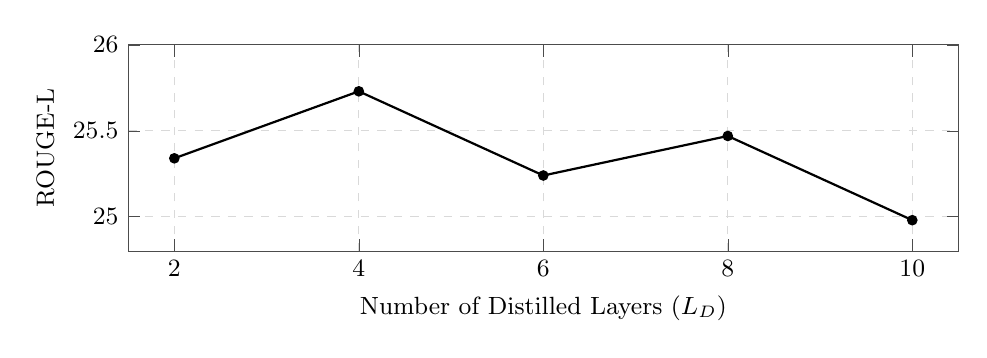
\begin{tikzpicture}
    \begin{axis}[
        xlabel={Number of Distilled Layers ($L_D$)},
        ylabel={ROUGE-L},
        width=\linewidth,
        height=4.2cm,
        xmin=1.5, xmax=10.5,
        ymin=24.8, ymax=26.0,
        xtick={2,4,6,8,10},
        ytick={25.0,25.5,26.0},
        grid=major,
        grid style={dashed, gray!30},
        axis line style={black!70},
        tick style={black!70},
        label style={font=\small},
        tick label style={font=\small},
        legend style={font=\small},
        every axis plot/.append style={
            thick,
            mark size=2.5pt
        }
    ]

    \addplot[
        color=black!70!black,
        mark=*,
        mark options={solid, fill=black!70!black},
        mark size = 1.5pt
    ] coordinates {
        (2, 25.34)
        (4, 25.73)
        (6, 25.24)
        (8, 25.47)
        (10, 24.98)
    };
    \end{axis}
\end{tikzpicture}%
} % Ends the resizebox
\captionof{figure}{Impact of the number of distilled layers $L_D$ on distillation performance.}
\label{fig:layer_ablation}
\end{minipage}
\subsection{Impact of Velocity Field Architecture}
\label{app:velofieldarch}
\begin{figure}[h]
\centering

\begin{subfigure}[t]{0.48\linewidth}
\centering
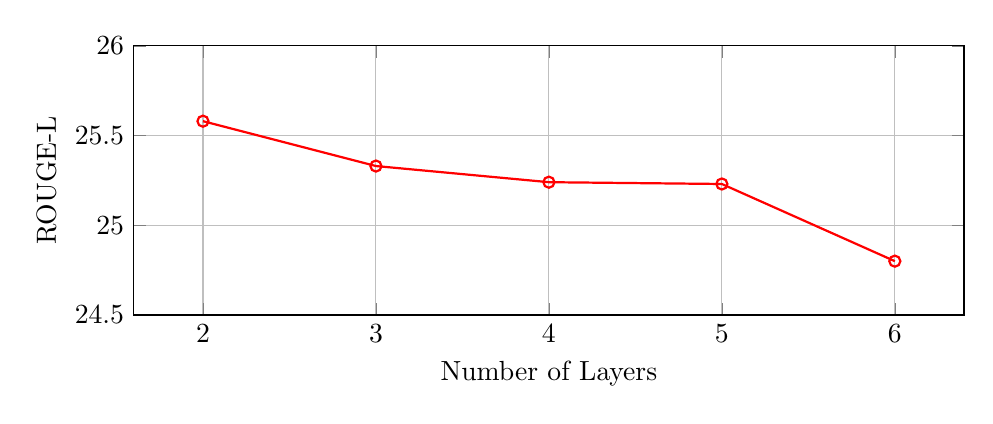
\begin{tikzpicture}
    \begin{axis}[
        xlabel={Number of Layers},
        ylabel={ROUGE-L},
        grid=major,
        width=\linewidth,
        height=5cm,
        xtick={2,3,4,5,6},
        ymin=24.5, ymax=26.0,
        mark options={solid},
        every axis plot/.append style={thick}
    ]
    \addplot[color=red, mark=o] coordinates {
        (2, 25.58)
        (3, 25.33)
        (4, 25.24)
        (5, 25.23)
        (6, 24.80)
    };
    \end{axis}
\end{tikzpicture}
\caption{Impact of velocity field's depth.}
\end{subfigure}
\hfill
\begin{subfigure}[t]{0.48\linewidth}
\centering
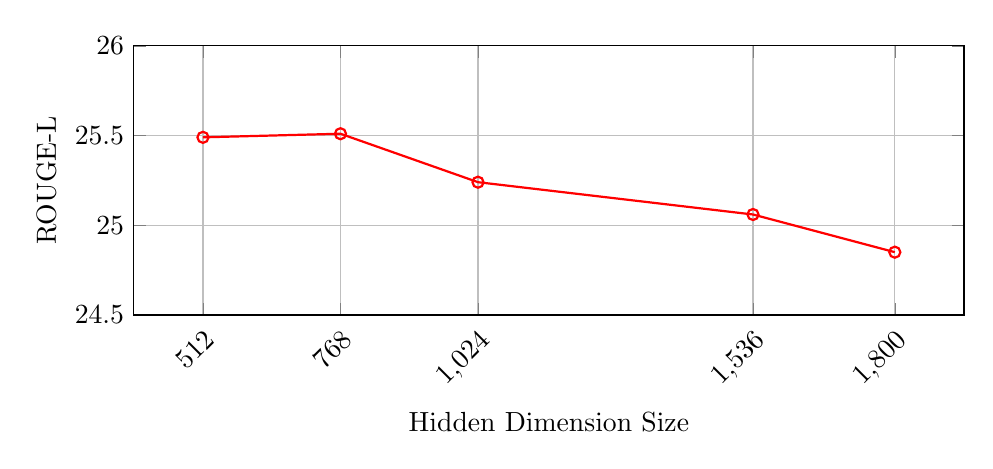
\begin{tikzpicture}
    \begin{axis}[
        xlabel={Hidden Dimension Size},
        ylabel={ROUGE-L},
        grid=major,
        width=\linewidth,
        height=5cm,
        xtick={512, 768, 1024, 1536, 1800},
        xticklabel style={rotate=45, anchor=north east},
        ymin=24.5, ymax=26.0,
        mark options={solid},
        every axis plot/.append style={thick}
    ]
    \addplot[color=red, mark=o] coordinates {
        (512, 25.49)
        (768, 25.51)
        (1024, 25.24)
        (1536, 25.06)
        (1800, 24.85)
    };
    \end{axis}
\end{tikzpicture}
\caption{Impact of velocity field's hidden dimension size.}
\end{subfigure}

\caption{Ablation study on the architecture of the velocity field. 
\textbf{Left:} Increasing the depth of the velocity field degrades distillation performance, indicating that the student--teacher trajectory mapping is smooth and does not require deep hierarchies. 
\textbf{Right:} The velocity field width must scale with the base model dimension; overly narrow networks introduce an information bottleneck and reduce feature transport fidelity.}
\label{fig:velocity_ablation}
\end{figure}
We analyze the impact of the velocity field architecture on distillation performance, focusing on two key design factors: model depth and hidden dimension. All experiments here are conducted using GPT2 1.5B $\rightarrow$ 0.1B pair with DistiLLM baseline and evaluation on the Dolly test set.

\paragraph{Impact of Velocity Field's depth.}
We examine the effect of network depth by varying the number of feed-forward blocks in the velocity field network $v_\theta$ from 2 to 6, while keeping the hidden dimension fixed at 1024. As shown in Figure~\ref{fig:velocity_ablation} (left), increasing the depth of the velocity field does not improve performance; instead, it leads to a gradual degradation. The highest ROUGE-L score of \textbf{25.58} is achieved with the shallowest configuration (2 layers), whereas the 6-layer model drops to 24.80. This trend suggests that the student-to-teacher trajectory mapping is relatively smooth and does not require deep hierarchical abstractions. A shallow and lightweight velocity field is therefore sufficient to model the feature transport, reinforcing the efficiency of our approach.

\paragraph{Impact of Velocity Field's hidden dimension.}
We investigate the effect of the velocity field width. Figure~\ref{fig:velocity_ablation} (right) shows the ROUGE-L scores for velocity fields with varying hidden dimensions. For the GPT2 setting (model dimension $d = 768$), compact velocity fields with comparable dimensionality perform best. However, when applying CONTRA-KD to larger language models (e.g., LLaMA2 13B $\rightarrow$ 7B (as shown in Table \ref{tab:velocity_dim_ablation}), where hidden dimensions exceed 4096), we observe that narrow velocity fields introduce a severe \emph{information bottleneck}. If the velocity field width is significantly smaller than the student or teacher hidden dimension, it fails to preserve the geometric structure of the feature manifold during projection, leading to degraded performance. These results indicate that the velocity field dimension should scale proportionally with the base model size in order to maintain faithful feature transport.

\begin{table}[h]
\caption{Impact of the velocity field's hidden dimension in LLaMA2 13B $\rightarrow$ 7B. ROUGE-L (\%) scores across different evaluation datasets, averaged over 5 random seeds.}
\label{tab:velocity_dim_ablation}
\begin{center}
\begin{small}
\begin{tabular}{lcccccc}
\toprule
Hidden Dimension Size & Dolly & Self-Inst & Vicuna & S-NI & UnNI & Avg. \\
\midrule
$d = 2048$ & 29.41 & 20.84 & 21.23 & \textbf{36.54} & 36.19 & 28.84 \\
$d = 3200$ & \textbf{31.45} & \textbf{23.69} & \textbf{21.48} & 36.19 & \textbf{37.70} & \textbf{30.10} \\
\bottomrule
\end{tabular}
\end{small}
\end{center}
\end{table}

\subsection{Velocity Field Architecture and Scaling}
\label{sec:appendix_low_rank_vf}

To address computational overhead when scaling CONTRA-KD to larger foundation models (e.g., beyond the 13B--7B parameter regime), the parameterization of the velocity field network $v_\theta$ can be optimized for lightweight inference and training. Specifically, standard dense projection layers in the velocity field can be replaced with a \textbf{low-rank projection architecture} (e.g., parameterizing intermediate feature transformations via low-rank factorizations).

To empirically verify that low-rank parameterization preserves continuous trajectory alignment without sacrificing representation fidelity, we evaluate a \textbf{Low-Rank Velocity Field (VF)} against our standard \textbf{Dense VF} baseline on the GPT-2 (1.5B $\rightarrow$ 0.1B) benchmark setup.

\begin{table}[htbp]
\centering
\small
\setlength{\tabcolsep}{4.5pt}
\caption{Ablation of velocity field architecture (Dense vs.\ Low-Rank projection) on GPT-2 (1.5B $\rightarrow$ 0.1B). ROUGE-L scores (\%) are averaged over 5 random seeds $\pm$ standard deviation.}
\label{tab:low_rank_vf_ablation}
\begin{tabular}{lcccccc}
\toprule
\textbf{Method} & \textbf{Dolly} & \textbf{Self-Inst} & \textbf{Vicuna} & \textbf{S-NI} & \textbf{UnNI} & \textbf{Avg.} \\
\midrule
Dense VF (Ours) & \textbf{26.22}$_{\pm 0.31}$ & \textbf{12.99}$_{\pm 0.53}$ & \textbf{17.41}$_{\pm 0.30}$ & \textbf{25.07}$_{\pm 0.21}$ & 26.85$_{\pm 0.11}$          & \textbf{21.71}$_{\pm 0.14}$ \\
Low-Rank VF     & 25.43$_{\pm 0.49}$          & 12.62$_{\pm 0.35}$          & 17.40$_{\pm 0.43}$          & 23.08$_{\pm 0.16}$          & \textbf{27.11}$_{\pm 0.10}$ & 21.13$_{\pm 0.15}$          \\
\bottomrule
\end{tabular}
\end{table}

As reported in Table~\ref{tab:low_rank_vf_ablation}, the low-rank design retains highly competitive performance across all instruction-following tasks, achieving an average ROUGE-L score of 21.13\% compared to 21.71\% for the dense architecture (a minor 0.58-point drop), while substantially reducing computational and memory overhead. Notably, performance on \textit{Vicuna} (17.40\% vs.\ 17.41\%) and \textit{UnNI} (27.11\% vs.\ 26.85\%) remains virtually identical or slightly improved.

This ablation confirms that the velocity field can be parameter-efficiently factorized without disrupting continuous flow modeling or trajectory continuity. While we leave exhaustive architectural optimization and automated architecture search for velocity fields to future work, these results demonstrate a practical path for scaling CONTRA-KD to foundation models exceeding 13B parameters.

% \section{Limitations}
% \paragraph{Limitations.} While CONTRA-KD demonstrates consistent improvements across diverse settings, it introduces additional computational overhead relative to standard distillation baselines. The primary source of this overhead is that the velocity field's parameter count scales quadratically with the teacher's hidden dimension. To manage this scaling in our current experiments (up to LLaMA2 13B → 7B), we set the internal hidden dimension of the velocity field to approximately 60\% of the teacher's dimension. As shown in our ablation studies detailed in \ref{app:velofieldarch}, this configuration strikes the optimal balance. A promising approach to further reduce this cost is to adopt an autoencoder-like design that decouples the velocity field's complexity from the teacher's hidden dimension. We leave this optimization as concrete directions for future work. 



\end{document}
